% Compile: pdflatex five_class_terrain_mp.tex  (twice, for cross-references)
% Requires IEEEtran.cls. Figure paths resolve to ../assets/ in this repository.
\documentclass[conference]{IEEEtran}

\usepackage[T1]{fontenc}

\usepackage{cite}
\usepackage{amsmath,amssymb}
\usepackage{graphicx}
\usepackage{booktabs}
\usepackage{multirow}
\usepackage{url}
\usepackage{xcolor}
\definecolor{cForest}{HTML}{006400}
\definecolor{cWater}{HTML}{0000FF}
\definecolor{cBuild}{HTML}{FF0000}
\definecolor{cBarren}{HTML}{D2B48C}
\definecolor{cAgri}{HTML}{90EE90}
\newcommand{\ckey}[2]{\raisebox{0.5pt}{\fcolorbox{black!55}{#1}{\rule{0pt}{4pt}\rule{4pt}{0pt}}}~#2}
\usepackage{tikz}
\usetikzlibrary{shapes.geometric,arrows.meta,positioning}

\graphicspath{{../assets/}{../assets/report_figs/}{../assets/paper_figs/}}

% This IEEEtran build does not define \linebreakand, which is what wraps the
% author block onto a second row of four.
\makeatletter
\providecommand{\linebreakand}{%
  \end{@IEEEauthorhalign}\hfill\mbox{}\par\mbox{}\hfill
  \begin{@IEEEauthorhalign}}
\makeatother

\begin{document}

\title{Five-Class Terrain Classification from Sentinel-2 Optical,
Texture and Sentinel-1 Radar Features Using Machine Learning in Google
Earth Engine, with Statewide External Validation over Madhya Pradesh}

\author{
\IEEEauthorblockN{Abhinav Kumar}
\IEEEauthorblockA{\textit{Department of Computer}\\
\textit{Science \& Engineering}\\
\textit{PDPM IIITDM}\\
Jabalpur, India\\
24bcs007@iiitdmj.ac.in}
\and
\IEEEauthorblockN{Aaditya Poddar}
\IEEEauthorblockA{\textit{Department of Computer}\\
\textit{Science \& Engineering}\\
\textit{PDPM IIITDM}\\
Jabalpur, India\\
24bcs002@iiitdmj.ac.in}
\and
\IEEEauthorblockN{Siddharth Ilayaraja}
\IEEEauthorblockA{\textit{Department of Computer}\\
\textit{Science \& Engineering}\\
\textit{PDPM IIITDM}\\
Jabalpur, India\\
24bcs292@iiitdmj.ac.in}
\and
\IEEEauthorblockN{Shivam Dubey}
\IEEEauthorblockA{\textit{Department of Computer}\\
\textit{Science \& Engineering}\\
\textit{PDPM IIITDM}\\
Jabalpur, India\\
23pcse03@iiitdmj.ac.in}
\linebreakand
\IEEEauthorblockN{Ashutosh Saxena}
\IEEEauthorblockA{\textit{Department of Computer}\\
\textit{Science \& Engineering}\\
\textit{PDPM IIITDM}\\
Jabalpur, India\\
24bcs041@iiitdmj.ac.in}
\and
\IEEEauthorblockN{Akshay Pandey}
\IEEEauthorblockA{\textit{Department of Computer}\\
\textit{Science \& Engineering}\\
\textit{PDPM IIITDM}\\
Jabalpur, India\\
drakshay@iiitdmj.ac.in}
\and
\IEEEauthorblockN{Aarav Jain}
\IEEEauthorblockA{\textit{Department of Computer}\\
\textit{Science \& Engineering}\\
\textit{PDPM IIITDM}\\
Jabalpur, India\\
24bcs004@iiitdmj.ac.in}
\and
\IEEEauthorblockN{Aniruddha\thanks{*Corresponding author: aniruddha\_phd@iiitdmj.ac.in}}
\IEEEauthorblockA{\textit{Department of Computer}\\
\textit{Science \& Engineering}\\
\textit{PDPM IIITDM}\\
Jabalpur, India\\
aniruddha\_phd@iiitdmj.ac.in}
}

\maketitle

\begin{abstract}
Land cover classification is the basis of environmental management,
resource assessment and urban planning. Our earlier work classified
vegetation against non-vegetation from Sentinel-2 red, near-infrared and
NDVI features over a campus-scale area of interest. This study extends
that framework in three directions: from two classes to five (Forest,
Water, Buildings, Barren Land and Agriculture), from a purely optical
feature set to a multi-sensor stack that adds grey-level co-occurrence
matrix (GLCM) texture and Sentinel-1 C-band radar, and from a
campus-scale accuracy assessment to an independent evaluation across all
48 districts of Madhya Pradesh. The dominant error in optical-only
classification is bare ground being reported as built-up, because bright
dry soil and concrete are near identical in Sentinel-2 reflectance. We
show by controlled ablation that texture repairs the precision half of
this confusion and radar repairs the recall half, together lifting
bare-ground recall from 7\% to 54\% and overall accuracy from 58.6\% to
73.9\%. A validated reduction of the feature stack from 27 to 19 bands
improved accuracy further rather than degrading it. Accuracy assessment
is performed exclusively against a high-confidence consensus of five
independent public products (WorldCover, Dynamic World, WorldCereal,
GHSL and OPERA DSWx), with all reference samples buffered at least
100~m from any training point; the project's own labels are used for
training only. Across 4{,}787 statewide reference samples, eXtreme
Gradient Boosting attained the best performance with 85.11\% overall
accuracy and a Kappa coefficient of 0.814 in the winter season. We
further report that overall accuracy falls from 94.3\% under a random
split to 79.2--91.5\% under a spatially blocked split and to
61.1--85.0\% under statewide external validation, so the validation
protocol moves the reported figure further than the choice of classifier
does. All processing is performed inside Google Earth
Engine.
\end{abstract}

\begin{IEEEkeywords}
Random Forest, Support Vector Machine, XGBoost, Google Earth Engine,
GLCM texture, Sentinel-1 SAR, external validation, land cover
classification
\end{IEEEkeywords}

\section{Introduction}

Reliable land cover information underpins ecological monitoring, urban
growth assessment, agricultural statistics and sustainable land
management \cite{ref1,ref3}. Accurate discrimination of vegetated,
built-up, bare and cultivated surfaces is therefore an important task in
remote sensing and geospatial analysis.

Conventional ground-based surveys are time-consuming, labour-intensive
and limited in spatial and temporal coverage. With the advancement of
Earth observation technologies, satellite remote sensing has become an
efficient and reliable approach for large-scale land cover monitoring
\cite{ref4}. Among the available missions, the Sentinel-2 constellation
of the European Space Agency provides high spatial resolution
multispectral imagery with frequent revisit capability and free global
accessibility \cite{ref4,ref5}, and the Sentinel-1 constellation
provides all-weather C-band synthetic aperture radar over the same
period \cite{ref20}.

Machine learning techniques have gained traction for remote sensing
classification because of their capacity for modelling complex
non-linear relationships between spectral features and land cover
classes \cite{ref7,ref8,ref9,ref10}. Platform-based solutions such as Google
Earth Engine (GEE) have made such workflows reproducible at scale by
combining petabyte-scale archives with server-side classifiers
\cite{ref11,ref12,ref13}.

Our earlier study established a two-class vegetation and non-vegetation
framework on this platform, using bands B4 and B8 together with NDVI,
and compared Random Forest, Support Vector Machine and XGBoost across
seasonal and cloud cover conditions. That framework reported accuracies
close to unity on a held-out split inside the study area, and 0.905 to
0.914 on a spatially disjoint external region of 240 samples per class.

Extending the same framework to an operational five-class product over
an entire state exposed three problems that a two-class campus-scale
study cannot observe, and this paper is an account of measuring and
addressing them.

First, the two-class problem is spectrally easy and the five-class
problem is not. Water absorbs near-infrared and Forest reflects it, so
both are separated by single-index contrasts that have been reliable for
forty years \cite{ref1,ref2}. Bare ground and built-up surfaces are not
separable this way at all. We measured red reflectance of 0.222 for
desert bare ground against 0.226 for built-up, and short-wave infrared
of 0.334 against 0.342. These are equal within noise, and a classifier
that sees only per-pixel colour has nothing to work with.

Second, the accuracy figures a study reports depend more on the
validation protocol than on the classifier. Labelled points are
collected in clusters, so neighbouring 10~m pixels from the same lake or
forest patch land on both sides of a random split, and each model is
then scored against near-duplicates of its own training rows
\cite{ref21,ref22}.

Third, cultivated land is the largest land type in Madhya Pradesh and it
is not spectrally stable. A field is green in winter and bare earth in
the pre-monsoon window, so an Agriculture class and a Barren Land class
exchange members between seasons, and any statewide product has to be
evaluated in more than one of them.

The main contributions of this study are as follows:

\begin{enumerate}
\item A multi-sensor feature stack combining Sentinel-2 reflectance,
bareness and built-up indices, GLCM texture and Sentinel-1 radar, with a
controlled ablation attributing the measured gain of each group.
\item A validated reduction of that stack from 27 to 19 bands, shown to
improve rather than degrade accuracy on independent evaluation samples.
\item An evaluation protocol that scores predictions exclusively against
a high-confidence consensus of five independent public products across
all 48 districts of Madhya Pradesh, with an enforced leakage buffer.
\item A comparative evaluation of five classifiers (Random Forest, SVM
with RBF kernel, XGBoost, CART and KNN) under that protocol in two
seasons.
\item A quantified account of how much the reported accuracy of a land
cover study depends on its validation protocol rather than on its
classifier.
\end{enumerate}

\section{Study Area}

The labelled training data for this study were collected across Jabalpur
district in central India, centred near $79.93^\circ$E,
$23.18^\circ$N. The district contains a mixture of dense deciduous
forest, perennial and seasonal water bodies, dense urban fabric of
Jabalpur city, exposed rocky and bare ground, and extensive cultivated
land, which makes it suitable for building a five-class labelled set.

The evaluation area is the whole of Madhya Pradesh, an area of
approximately 308{,}776~km\textsuperscript{2} spanning roughly
$74.0^\circ$E to $82.8^\circ$E. The state was partitioned by its 48
administrative districts as defined by the FAO GAUL level-2 boundaries.
This region is deliberately far larger and more varied than the training
area. It contains the black cotton soils of the Malwa plateau, the
ravines of the Chambal valley, the dry rocky terrain of Bundelkhand, and
the humid forested belt of the Satpura range, none of which has a
counterpart in the Jabalpur training set. Evaluating on it therefore
measures spatial generalisation rather than interpolation, which is the
property an operational product needs.

\section{Methodology}

Fig.~\ref{fig:workflow} shows the overall workflow through sequential
processing stages, from data acquisition to accuracy assessment and the
final classified map output.

\begin{figure*}[!t]
\centering
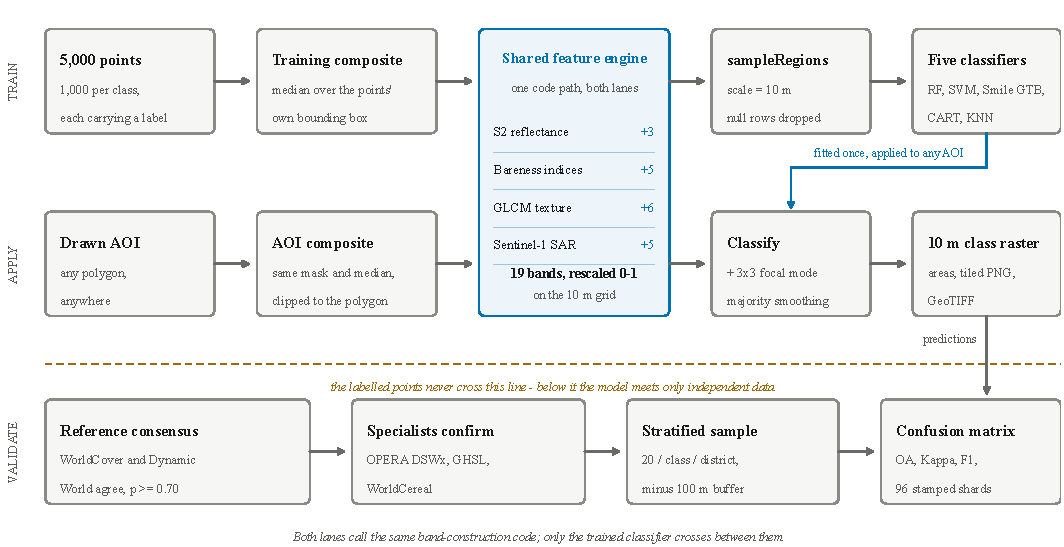
\includegraphics[width=\textwidth]{fig_pipeline.pdf}
\caption{Five-class terrain classification pipeline. The training lane fits a classifier on the labelled points inside Jabalpur and the inference lane applies it to any drawn area; both call the same band-construction code, so a training pixel and an inference pixel cannot be built differently. The only quantity crossing between the lanes is the trained classifier, and the only quantity crossing into the evaluation lane is a prediction: the labelled points are never scored against.}
\label{fig:workflow}
\end{figure*}

\subsection{Data Acquisition}

The optical dataset used in this study was Sentinel-2 Level-2A surface
reflectance imagery, retrieved from Google Earth Engine using the image
collection \texttt{COPERNICUS/S2\_SR\_HARMONIZED}. Images were filtered
by the spatial extent of the region being processed and by acquisition
date, and scenes with \texttt{CLOUDY\_PIXEL\_PERCENTAGE} of 15\% or
greater were discarded so that atmospheric disturbance and cloud
contamination are minimised. Where a district and season combination
returned no scene under that threshold, the filter was relaxed to 30\%
rather than allowing an empty composite.

The radar dataset was Sentinel-1 Ground Range Detected imagery from
\texttt{COPERNICUS/S1\_GRD}, restricted to Interferometric Wide swath
mode and to scenes carrying both VV and VH polarisations.

Two seasonal windows were fixed for all experiments, both in 2025 and
both with exclusive end dates: winter from 2025-01-01 to 2025-02-28, and
summer from 2025-03-31 to 2025-04-30. Fixing the windows is necessary
because otherwise a seasonal comparison also varies the composite depth.

\subsection{Cloud Masking and Image Preprocessing}

Clouds and atmospheric effects corrupt the spectral reflectance values
on which classification depends. Each retained image was therefore
processed using the Quality Assessment (QA60) bit mask band. Bits 10
(opaque clouds) and 11 (cirrus cloud) were used to generate a binary
mask:

\begin{equation}
M(x,y) = \overline{Q_{10}(x,y)} \wedge \overline{Q_{11}(x,y)}
\end{equation}

where $Q_{10}$ and $Q_{11}$ denote the respective QA60 bit values at
pixel $(x,y)$. Masked pixels were excluded from the subsequent median
composite. After masking, all pixel values were scaled by a factor of
$1/10{,}000$ to convert from digital numbers to physical reflectance
units.

The Sentinel-1 collection was reduced by a per-pixel temporal median
over the same window. Backscatter is rescaled from decibels into the
approximate interval $[0,1]$, with VV mapped from $[-25,5]$~dB and VH
from $[-30,0]$~dB. This rescaling is not cosmetic. The SVM classifier
uses a radial basis function kernel, which is distance-based, and raw
decibel values spanning $-25$ to $5$ would otherwise dominate every
reflectance feature in the kernel.

\subsection{Feature Extraction}

Table~\ref{tab:bands} lists the nineteen features that form the
classifier input. Several further quantities are computed as
intermediates and are not themselves presented to the classifier: bands
B2, B4 and B8 and the indices NDVI, NDWI, NDBI and SAVI enter only
through the retained indices defined below.
Section~\ref{sec:bandcut} reports the evidence for excluding them.

The bareness and built-up group targets the confusion that no vegetation
contrast can address. The Bare Soil Index \cite{ref26} is

\begin{equation}
\mathrm{BSI} = \frac{(B11 + B4) - (B8 + B2)}{(B11 + B4) + (B8 + B2)}
\end{equation}

and the Index-based Built-up Index \cite{ref27} combines NDBI
\cite{ref24}, SAVI \cite{ref28} and MNDWI \cite{ref25} in the form

\begin{equation}
\mathrm{IBI} = \frac{2\,\mathrm{NDBI} - (\mathrm{SAVI} + \mathrm{MNDWI})}
                    {2\,\mathrm{NDBI} + (\mathrm{SAVI} + \mathrm{MNDWI})}
\end{equation}

Six Haralick texture measures \cite{ref23} were computed on the
near-infrared band, quantised to 32 grey levels, using the GEE
\texttt{glcmTexture()} reducer: contrast, entropy, variance, inverse
difference moment, dissimilarity and angular second moment. Contrast and
variance were computed on the same basis from the VV channel.

\begin{table}[!t]
\caption{The nineteen features presented to the classifier}
\label{tab:bands}
\centering
\footnotesize
\begin{tabular}{@{}p{19mm}p{36mm}p{13mm}@{}}
\toprule
\textbf{Group} & \textbf{Features} & \textbf{Resolution} \\
\midrule
S-2 reflectance & B3, B11, B12 & 10--20 m \\
Bareness / built-up & BSI, UI, IBI, SWIRratio, BAEI & 10--20 m \\
GLCM texture (B8) & g\_contrast, g\_ent, g\_var, g\_idm, g\_diss, g\_asm & 10 m \\
S-1 backscatter & VV, VH, VV/VH ratio & 10 m \\
GLCM texture (VV) & s\_contrast, s\_var & 10 m \\
\bottomrule
\end{tabular}
\end{table}

Texture and radar are present for one reason, and it is physical rather
than statistical. Built-up surfaces are structurally rough at the scale
of a few pixels because of edges, roof lines and shadows, whereas bare
soil is smooth; that is information no single pixel carries, and texture
is how it enters the model. Independently, buildings produce a
double-bounce return from wall and ground surfaces that bare soil cannot
imitate at any brightness, and that mechanism is visible to radar and
invisible to any optical band.

\subsection{Training Data Preparation}

Five classes were labelled with contiguous integer labels: Forest 0,
Water 1, Buildings 2, Barren Land 3 and Agriculture 4. One thousand
manually collected point features were prepared per class, giving 5{,}000
labelled points. Pixel values for the selected features were extracted
using the \texttt{sampleRegions()} function in Google Earth Engine, and
the training composite geometry was derived from the bounding box of the
labelled points themselves so that no labelled point can fall outside
the composite.

Label integrity is enforced rather than assumed, because the failure mode
here is silent. \texttt{sampleRegions(properties=['label'])} drops rows
whose label property is null without raising, so a point collection that
has lost its attributes contributes zero training rows and the model
simply trains on fewer classes than were configured, with no error
anywhere in the pipeline. Every source asset therefore carries its own
label attribute, so class identity travels with the points, and a
pre-training audit asserts the expected label histogram and point count
per asset before any run. A schema version string is stamped into every
stored result, so results computed under different class inventories
cannot be merged.

\subsection{Machine Learning Classification Algorithms}

Five supervised classifiers were implemented and compared, all
server-side in Google Earth Engine, with the parameters listed in
Table~\ref{tab:models}.

\begin{enumerate}
\item \textit{Random Forest}: an ensemble that builds multiple decision
trees and classifies by majority vote \cite{ref15}, implemented with
\texttt{ee.Classifier.smileRandomForest}.
\item \textit{Support Vector Machine}: locates the optimal separating
boundary in feature space \cite{ref16}, here with a radial basis
function kernel, implemented with \texttt{ee.Classifier.libsvm}.
\item \textit{XGBoost}: an ensemble that applies weak decision trees
sequentially, each correcting the errors of its predecessors
\cite{ref17}, implemented with
\texttt{ee.Classifier.smileGradientTreeBoost}.
\item \textit{CART}: a single classification and regression tree,
implemented with \texttt{ee.Classifier.smileCart}.
\item \textit{KNN}: majority vote among the $k$ nearest training samples
in feature space, implemented with \texttt{ee.Classifier.smileKNN}.
\end{enumerate}

\begin{table}[!t]
\caption{Classifier configurations, shared by the notebooks, the
evaluation harness and the served model}
\label{tab:models}
\centering
\footnotesize
\begin{tabular}{@{}ll@{}}
\toprule
\textbf{Classifier} & \textbf{Parameters} \\
\midrule
Random Forest & 200 trees, bag fraction 0.3, maxNodes 10 \\
SVM & RBF kernel, $\gamma=1.0$, cost 100 \\
XGBoost & 100 trees, shrinkage 0.1, maxNodes 10 \\
CART & maxNodes 20 \\
KNN & $k=5$ \\
\bottomrule
\end{tabular}
\end{table}

\subsection{Independent Reference Construction and Accuracy Assessment}
\label{sec:reference}

A land cover study that scores its models on held-out points drawn from
its own labelled set measures how well the model reproduces the
annotator, not how well it maps the terrain. We therefore adopted a
strict separation: the project's manually labelled points are used for
training only, and every reported accuracy figure is agreement with an
independent reference constructed from public products.

The reference is a high-confidence consensus. ESA WorldCover
\cite{ref18} and Dynamic World \cite{ref19} must agree on a pixel before
it is admitted, and the Dynamic World class probability must exceed 0.70.
Specialist products then confirm three of the five classes: OPERA DSWx
confirms Water, the Global Human Settlement Layer built surface product
confirms Buildings at a threshold of 50~m\textsuperscript{2} per 10~m
cell, and WorldCereal \cite{ref29} confirms Agriculture. A pixel labelled
Bare by both general products is admitted only where none of the three
specialist products claims it. Every pixel failing any of these tests is
masked out of the reference entirely rather than being assigned a
best-guess class.

Sampling was stratified: 20 points per reference class per district, at
10~m scale, across all 48 districts. Any candidate sample falling within
100~m of any training point was then removed by an inverted spatial
join, so no reference sample can sit on a pixel neighbouring a training
pixel. After this buffer, 4{,}787 samples remained for the winter
evaluation and 4{,}627 for summer, distributed across all 48 districts.

Overall Accuracy and the Kappa coefficient \cite{ref30} were computed,
together with per-class precision, recall and F1. Overall Accuracy
indicates the proportion of correctly labelled samples, while Kappa
evaluates agreement beyond random chance.

\subsection{Google Earth Engine Platform}

All preprocessing, feature extraction, training, classification and
accuracy assessment were performed inside the Google Earth Engine cloud
environment \cite{ref11}. A single statewide request exceeds the
interactive compute limit, so the evaluation was sharded into 96 units
of one district and one season, each independently checkpointed and each
stamped with the schema version of the class inventory under which it was
computed. A shard stamped with a different schema version is refused by
the aggregator rather than merged, which is what makes a statewide
figure assembled from 96 separate computations trustworthy.

\section{Experimental Results and Discussion}

\subsection{Attribution of Each Feature Group}

The contribution of each feature group was measured separately against
the original ten-band optical baseline, with Random Forest, on 1{,}274
evaluation points across Madhya Pradesh. No labels were added at any
stage of this ablation, so every difference in Table~\ref{tab:ablation}
is attributable to features alone.

\begin{table}[!t]
\caption{Feature group attribution, Random Forest, 1{,}274 statewide
evaluation points. The final column counts bare-ground samples
misclassified as Buildings.}
\label{tab:ablation}
\centering
\footnotesize
\begin{tabular}{@{}lcccc@{}}
\toprule
\textbf{Feature set} & \textbf{Overall} & \textbf{Bare recall} &
\textbf{Built prec.} & \textbf{Bare$\rightarrow$Built} \\
\midrule
Baseline, 10 bands      & 58.6\% & 7\%  & 49\% & 213 \\
+ bareness indices      & 60.4\% & 11\% & 51\% & 203 \\
+ GLCM texture          & 65.3\% & 37\% & 58\% & 130 \\
+ Sentinel-1 SAR        & 70.6\% & 50\% & 59\% & 91  \\
\textbf{All 27 features} & \textbf{73.9\%} & \textbf{54\%} & \textbf{63\%} & \textbf{83} \\
\bottomrule
\end{tabular}
\end{table}

Three results in this table deserve comment.

The bareness and built-up indices contributed least, at 1.8 percentage
points. This is the expected outcome and it is a negative result worth
recording: NDBI, UI and IBI were designed to separate built-up from
vegetation, not built-up from bare soil, and in dry scenes bare soil
ranks above built-up in all three \cite{ref24,ref31}. They are algebraic
rearrangements of bands the classifier already had, so a non-linear
model can largely represent them internally. Adding more indices of this
family cannot repair this confusion.

GLCM texture moved Buildings precision from 51\% to 58\%, and cut the
bare-to-built error from 203 to 130. It fixed the precision half of the
confusion, because it stops smooth surfaces being called buildings.

Sentinel-1 radar moved bare-ground recall from 7\% to 50\% on its own,
the largest single jump in this study. It fixed the recall half, because
double-bounce is a scattering mechanism rather than an appearance.

Texture and radar therefore attack opposite halves of the same
confusion, which is why using both exceeds either alone.

Fig.~\ref{fig:attribution} measures the same question by removal rather
than by addition, which avoids crediting whichever family happens to be
added first with everything two families share. The ranking is
unambiguous: Sentinel-1 amplitude is the one family the stack cannot
lose, and the core indices are the one family it is measurably better
without.

\begin{figure*}[!t]
\centering
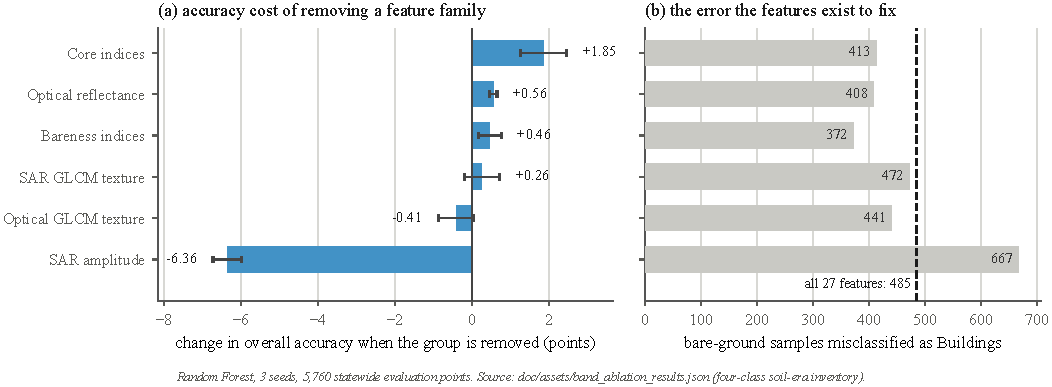
\includegraphics[width=\textwidth]{fig_group_attribution.pdf}
\caption{Contribution of each feature family, measured by removal from the 27-band stack. (a) change in overall accuracy when the family is dropped; bars left of zero are families the model needs. (b) the bare-ground-to-Buildings confusion the texture and radar families exist to reduce, against the all-features reference. Error bars are the standard error over seeds.}
\label{fig:attribution}
\end{figure*}

\subsection{Reduction from 27 Bands to 19}
\label{sec:bandcut}

Adding features is not monotonically beneficial. Two reduced stacks were
evaluated against the full 27-band stack on 5{,}760 independent
evaluation points, over nine random seeds for Random Forest and five for
XGBoost. The 22-band cut drops B8, NDVI, NDWI, NDBI and s\_ent; the
19-band cut additionally drops B2, B4 and SAVI.
Table~\ref{tab:bandcut} reports the outcome.

\begin{table}[!t]
\caption{Effect of reducing the feature stack, 5{,}760 independent
evaluation points, mean over seeds}
\label{tab:bandcut}
\centering
\footnotesize
\begin{tabular}{@{}lcccc@{}}
\toprule
\textbf{Classifier} & \textbf{Bands} & \textbf{Overall} &
\textbf{Kappa} & \textbf{Bare$\rightarrow$Built} \\
\midrule
\multirow{3}{*}{Random Forest}
 & 27 & 72.85\% & 0.638 & 474.7 \\
 & 22 & 74.28\% & 0.657 & 432.8 \\
 & \textbf{19} & \textbf{77.33\%} & \textbf{0.697} & \textbf{378.4} \\
\midrule
\multirow{3}{*}{XGBoost}
 & 27 & 73.57\% & 0.646 & 365.0 \\
 & 22 & 73.60\% & 0.647 & 355.4 \\
 & \textbf{19} & \textbf{74.62\%} & \textbf{0.660} & \textbf{352.4} \\
\midrule
\multirow{3}{*}{SVM (RBF)}
 & 27 & 73.20\% & 0.642 & 417.0 \\
 & 22 & 74.06\% & 0.653 & 392.0 \\
 & \textbf{19} & \textbf{74.42\%} & \textbf{0.658} & 417.0 \\
\bottomrule
\end{tabular}
\end{table}

The 19-band cut is better than the full stack for every classifier, by
4.5 points for Random Forest, 1.0 for Gradient Boosting and 1.2 for SVM,
and the improvement is far larger than the seed-to-seed standard error,
which stays below 0.19 percentage points on every row. The bands removed are the ones
whose information is already carried by a retained band or by an index
computed from them, and removing them reduces the correlated-feature
dilution that hurts bagged trees.

This result was confirmed on a geographically held-out design. Features
were selected on the western half of the state and the stacks were then
scored only on the eastern half, on 2{,}880 samples never used for
selection. The 19-band cut led there as well, at 80.50\% overall and
0.740 Kappa, against 77.42\% and 0.699 for the full 27-band stack, which
establishes that the reduction is not an artefact of selecting and
scoring on the same terrain. All results reported below use the 19-band
stack. Fig.~\ref{fig:bandcut} plots the three stacks against each other
with their seed-to-seed error.

\begin{figure}[!t]
\centering
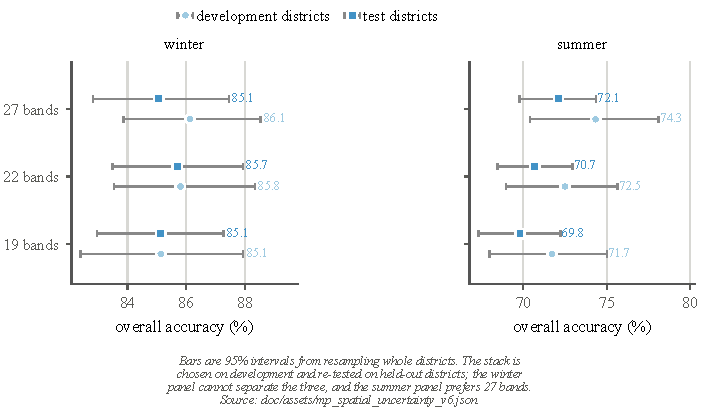
\includegraphics[width=\columnwidth]{fig_band_cut.pdf}
\caption{Overall accuracy of the 27-, 22- and 19-band stacks for three classifiers, mean over seeds with standard error. Plotted as positions rather than bar lengths because the spread is a few points on a 0--100 scale. For XGBoost the 27- and 22-band markers coincide.}
\label{fig:bandcut}
\end{figure}

\subsection{Comparative Analysis of the Classifiers}
\label{sec:models}

Table~\ref{tab:models_ext} reports the statewide external performance of
all five classifiers under the current inventory, and
Fig.~\ref{fig:models} shows the same figures with the seasonal gap made
visible.

\begin{figure}[!t]
\centering
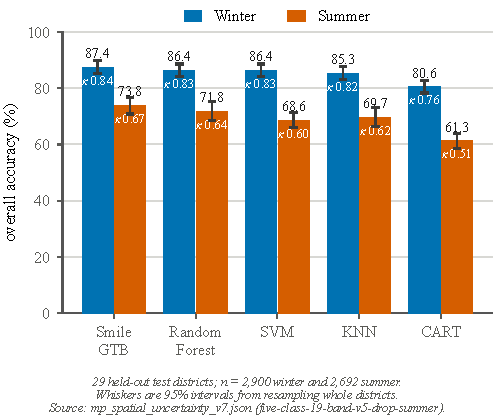
\includegraphics[width=\columnwidth]{fig_model_comparison.pdf}
\caption{Statewide external accuracy of the five classifiers in both validated seasons, with the Kappa coefficient inset in each bar. Every value is agreement with the public-map consensus over 48 districts, not a held-out split of the project's own labels.}
\label{fig:models}
\end{figure}

\begin{table}[!t]
\caption{Statewide external accuracy, 48 districts, 4{,}787 winter and
4{,}627 summer reference samples}
\label{tab:models_ext}
\centering
\footnotesize
\begin{tabular}{@{}lcccc@{}}
\toprule
\multirow{2}{*}{\textbf{Classifier}} &
\multicolumn{2}{c}{\textbf{Winter}} &
\multicolumn{2}{c}{\textbf{Summer}} \\
\cmidrule(lr){2-3}\cmidrule(lr){4-5}
 & \textbf{OA} & \textbf{Kappa} & \textbf{OA} & \textbf{Kappa} \\
\midrule
\textbf{XGBoost}    & \textbf{85.11\%} & \textbf{0.814} & \textbf{70.30\%} & \textbf{0.627} \\
SVM (RBF)           & 84.10\% & 0.801 & 69.70\% & 0.619 \\
KNN ($k=5$)         & 83.16\% & 0.790 & 65.25\% & 0.563 \\
Random Forest       & 78.04\% & 0.726 & 61.96\% & 0.521 \\
CART                & 71.36\% & 0.642 & 61.14\% & 0.511 \\
\bottomrule
\end{tabular}
\end{table}

XGBoost leads on every aggregate metric in both seasons, but narrowly:
by 1.01 percentage points over SVM in winter and 0.60 in summer. Two
classifiers exceed 0.80 Kappa in winter and a third reaches 0.797.

An earlier version of this comparison placed SVM and KNN last, at
71.34\% and 73.68\% in winter, and attributed the gap to an RBF
$\gamma$ of 1.0 inherited from a lower-dimensional problem. That
diagnosis was wrong, and the true cause is worth reporting because it is
invisible in the accuracy figures themselves. The GLCM texture moments
were entering the feature stack in their native units while every other
band lay in $[0,1]$ or $[-1,1]$; on a 32-level composite, raw GLCM
variance reaches 143. Measured across the training samples, the four
widest texture bands accounted for 97\% of the squared Euclidean
distance between feature vectors, and variance alone for 51\%. A
threshold-based learner is invariant to any monotonic rescaling of a
single feature, so CART, Random Forest and XGBoost were untouched by
this, but an RBF kernel and a $k$-nearest-neighbour search operate on
precisely that distance, and both were therefore being fitted almost
entirely on two texture bands with the optical and radar evidence
contributing almost nothing.

Rescaling every band to a common $[0,1]$ range, with bounds set at the
99th percentile so that heavy tails do not compress the informative part
of the range into a fraction of the scale, moves SVM by 12.76 percentage
points and KNN by 9.48 in winter, and by 8.56 and 3.91 in summer, at an
unchanged $\gamma$ of 1.0. The three tree models move by at most 0.15
points, the residue of the clamp tying the top 1\% of texture values
together and removing the few splits that lived inside that tail. The
earlier ranking was thus a statement about preprocessing rather than
about the algorithms. The methodological point generalises: a comparison
between distance-based and threshold-based classifiers is
uninterpretable unless feature scaling has been verified, because an
unscaled stack degrades only half of the table and the result reads as a
genuine algorithmic difference rather than as a defect.

Sequential boosting has a specific advantage on this problem. The
residual errors after the easy classes are resolved are concentrated in
one confusion, bare against built-up, and boosting reweights precisely
towards the samples that previous trees misclassified. Bagged ensembles
distribute effort uniformly instead. Consistently with this, XGBoost
attains the best Bare F1 of any classifier in both seasons, at 0.753 and
0.551.

\subsection{Per-Class Performance and the Remaining Error}

Table~\ref{tab:perclass} reports per-class F1 in both seasons, and
Fig.~\ref{fig:perclassfig} shows the same values as a heat map, in which
the column structure is easier to read than the row structure: the choice
of classifier barely moves Water and moves Bare a great deal.
\begin{figure*}[!t]
\centering
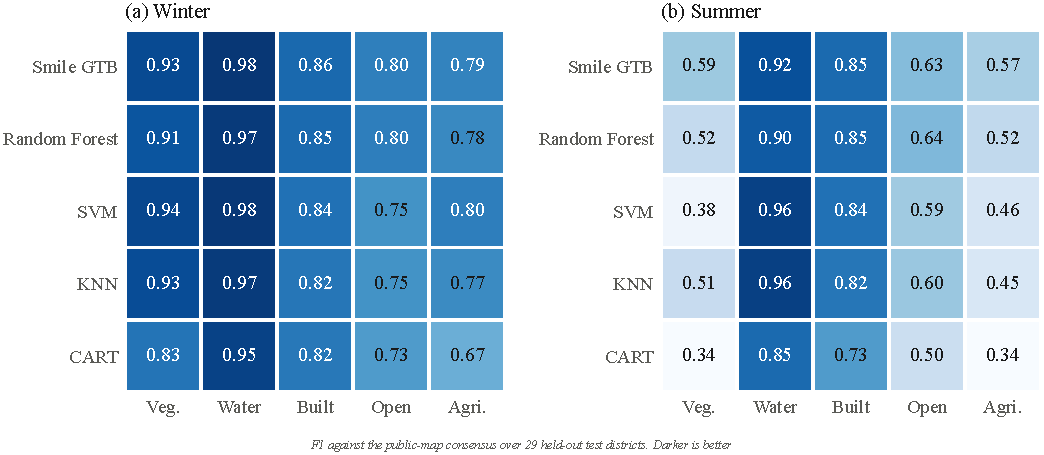
\includegraphics[width=\textwidth]{fig_per_class_f1.pdf}
\caption{Per-class F1 for every classifier under the statewide external reference. (a) Winter. (b) Summer. Darker is better; values are printed in every cell so the encoding is never colour alone.}
\label{fig:perclassfig}
\end{figure*}

\begin{table}[!t]
\caption{Per-class F1 under the statewide external reference}
\label{tab:perclass}
\centering
\footnotesize
\setlength{\tabcolsep}{3.4pt}
\begin{tabular}{@{}llccccc@{}}
\toprule
\textbf{Season} & \textbf{Classifier} & \textbf{Forest} & \textbf{Water} &
\textbf{Buildings} & \textbf{Bare} & \textbf{Agri.} \\
\midrule
\multirow{5}{*}{Winter}
 & XGBoost       & 0.916 & 0.961 & \textbf{0.839} & \textbf{0.753} & 0.771 \\
 & Random Forest & 0.840 & \textbf{0.969} & 0.749 & 0.654 & 0.647 \\
 & KNN           & 0.899 & 0.960 & 0.812 & 0.727 & 0.736 \\
 & CART          & 0.834 & 0.951 & 0.635 & 0.452 & 0.654 \\
 & SVM (RBF)     & \textbf{0.930} & 0.957 & 0.821 & 0.687 & \textbf{0.786} \\
\midrule
\multirow{5}{*}{Summer}
 & XGBoost       & 0.589 & 0.883 & \textbf{0.854} & \textbf{0.551} & \textbf{0.536} \\
 & Random Forest & 0.294 & 0.923 & 0.815 & 0.421 & 0.422 \\
 & KNN           & 0.434 & 0.932 & 0.821 & 0.525 & 0.417 \\
 & CART          & 0.314 & 0.919 & 0.795 & 0.367 & 0.439 \\
 & SVM (RBF)     & \textbf{0.616} & \textbf{0.935} & 0.830 & 0.481 & 0.533 \\
\bottomrule
\end{tabular}
\end{table}

\begin{figure*}[!t]
\centering
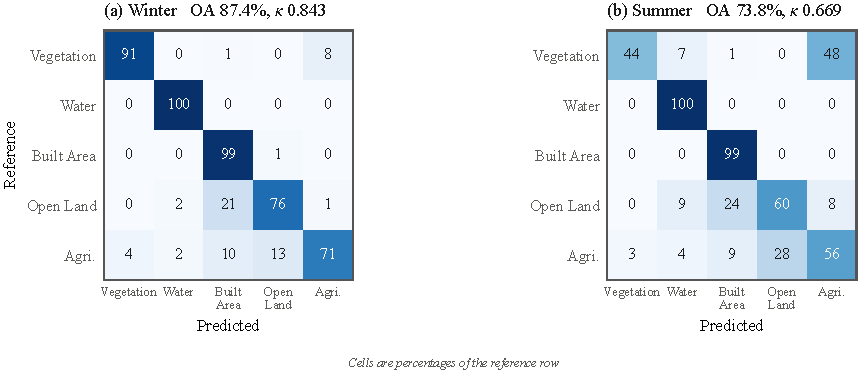
\includegraphics[width=\textwidth]{fig_confusion_seasonal.pdf}
\caption{XGBoost confusion matrices under the statewide external
reference, row-normalised to percentages. (a) Winter. (b) Summer, in
which Forest recall falls from 87\% to 43\% under leaf-off dry deciduous
canopy, and Agriculture and Bare exchange members in both directions as
cultivated fields lie fallow.}
\label{fig:seasonal}
\end{figure*}

The class ordering is identical for every classifier, which is the
clearest single indication that the residual difficulty is set by the
data and the class definitions rather than by the choice of algorithm.

Water is the strongest class throughout, with winter F1 between 0.95 and
0.97 for all five classifiers, because open water is close to black in
the near-infrared and is spectrally unambiguous. Under the unscaled
stack described above SVM was the single exception at 0.759, and the
failure was one of precision rather than recall: recall was 1.00 against
a precision of 0.61, visible in the product as dense urban fabric
reported as water. Rescaling lifts that precision to 0.92 and the F1 to
0.957, which is the clearest single confirmation that the defect lay in
the feature representation and not in the kernel.

Forest follows at 0.83 to 0.93 in winter. Bare and Agriculture are the
weakest classes for every classifier, and they are weak together, which
is the signature of a single shared difficulty rather than two
independent ones.

The seasonal half of the table shows what that difficulty is.
Fig.~\ref{fig:seasonal} places the two XGBoost confusion matrices side by
side. In winter, 13\% of Agriculture reference samples are called Bare
and 3\% of Bare is called Agriculture; in summer those leaks grow to
31\% and 17\%. The summer composite falls in the pre-monsoon fallow
period, when a cultivated field in central India is bare earth, so the
two classes are not merely harder to tell apart, they are physically the
same surface at that date. Forest degrades for the mirror-image reason:
recall falls from 0.87 in winter to 0.43 in summer as leaf-off dry
deciduous canopy over dry ground reads as bare ground. Buildings is the
only class that is stable across seasons, at 0.839 and 0.854 under
XGBoost, which is consistent with built-up being the one surface whose
scattering behaviour does not follow phenology. A single-date statewide
product should therefore be built on a winter composite, and any
Agriculture figure quoted from a pre-monsoon composite should be treated
as unreliable.

Fig.~\ref{fig:indore} shows the same failure on the ground rather than
in a matrix. Over the Indore fringe the built-up class spreads well
beyond the visibly built fabric into the dry open ground around it. That
over-extension is the same error the confusion matrices count, seen at
the scale a user of the map actually works at.

Fig.~\ref{fig:seasonal}(a) also shows where the residual error sits. The
dominant off-diagonal cell remains bare ground reported as built-up.
Texture and radar reduce this confusion substantially, as
Table~\ref{tab:ablation} shows, but do not eliminate it. The indices in
the literature that do separate the two materials reliably require a
thermal band, which Sentinel-2 does not carry, so part of what remains is
a sensor ceiling rather than an engineering gap.

Fig.~\ref{fig:beforeafter} isolates what the move to the five-class
inventory changed, with both conditions scored against the identical
reference. Only two classes move: Bare gains 0.22 F1 from the Barren Land
labels, and Agriculture goes from a class the earlier inventory could not
predict at all to 0.77. Forest, Water and Buildings shift by at most
0.008, which is what makes the comparison credible.

\begin{figure}[!t]
\centering
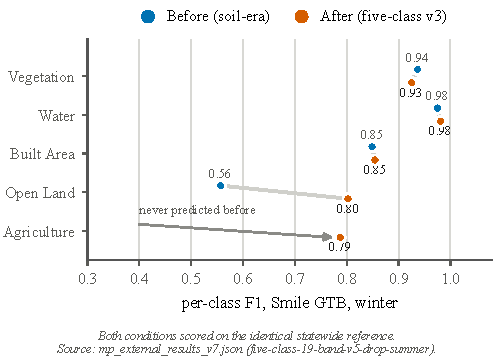
\includegraphics[width=\columnwidth]{fig_before_after.pdf}
\caption{Per-class F1 before and after the move to the five-class inventory, XGBoost, winter, both conditions scored on the identical statewide reference. The two conditions are dodged onto separate rows because three of the five classes move by less than 0.01.}
\label{fig:beforeafter}
\end{figure}

\subsection{Spatial Generalisation}
\label{sec:spatial}

Accuracy is not uniform across the state, and it decays with distance
from the labelled area. A tile-based analysis over Madhya Pradesh shows
overall accuracy rising monotonically from 62\% in the westernmost tile
column to 76\% in the easternmost, approaching the
$79.4^\circ$--$80.6^\circ$E band that the training points occupy. The
weakest terrain is the Malwa plateau and the Chambal ravines in the
north-west, whose black cotton soil, bare rock and bright dry fallow
have no counterpart in the Jabalpur training set; the strongest is the
forested Satpura belt, whose terrain the training points do represent.
The gradient is therefore a map of where the training distribution is
thin rather than a property of any classifier, and all five degrade
along it together.

The size of this effect was measured directly by adding labels rather
than by changing the model. A configuration carrying 1{,}000
bare-ground labels distributed across the state, instead of labels drawn
from Jabalpur alone, raised statewide bare-ground recall from 7\% to
54\%. At the far edge of the gradient, over the Thar dune field, that
configuration reported 85.3\% bare ground and 13.9\% built-up under
Random Forest against a reference of 422{,}453~ha bare and 2{,}216~ha
built, where the Jabalpur-only configuration had read the same terrain
as 80.9\% Buildings. Labelling the unrepresented terrain is what closed
that gap, and no feature or hyperparameter change in this study
approached it.

\subsection{Effect of the Validation Protocol}

Table~\ref{tab:protocol} reports the same models under three validation
protocols of increasing strictness.

\begin{figure*}[!t]
\centering
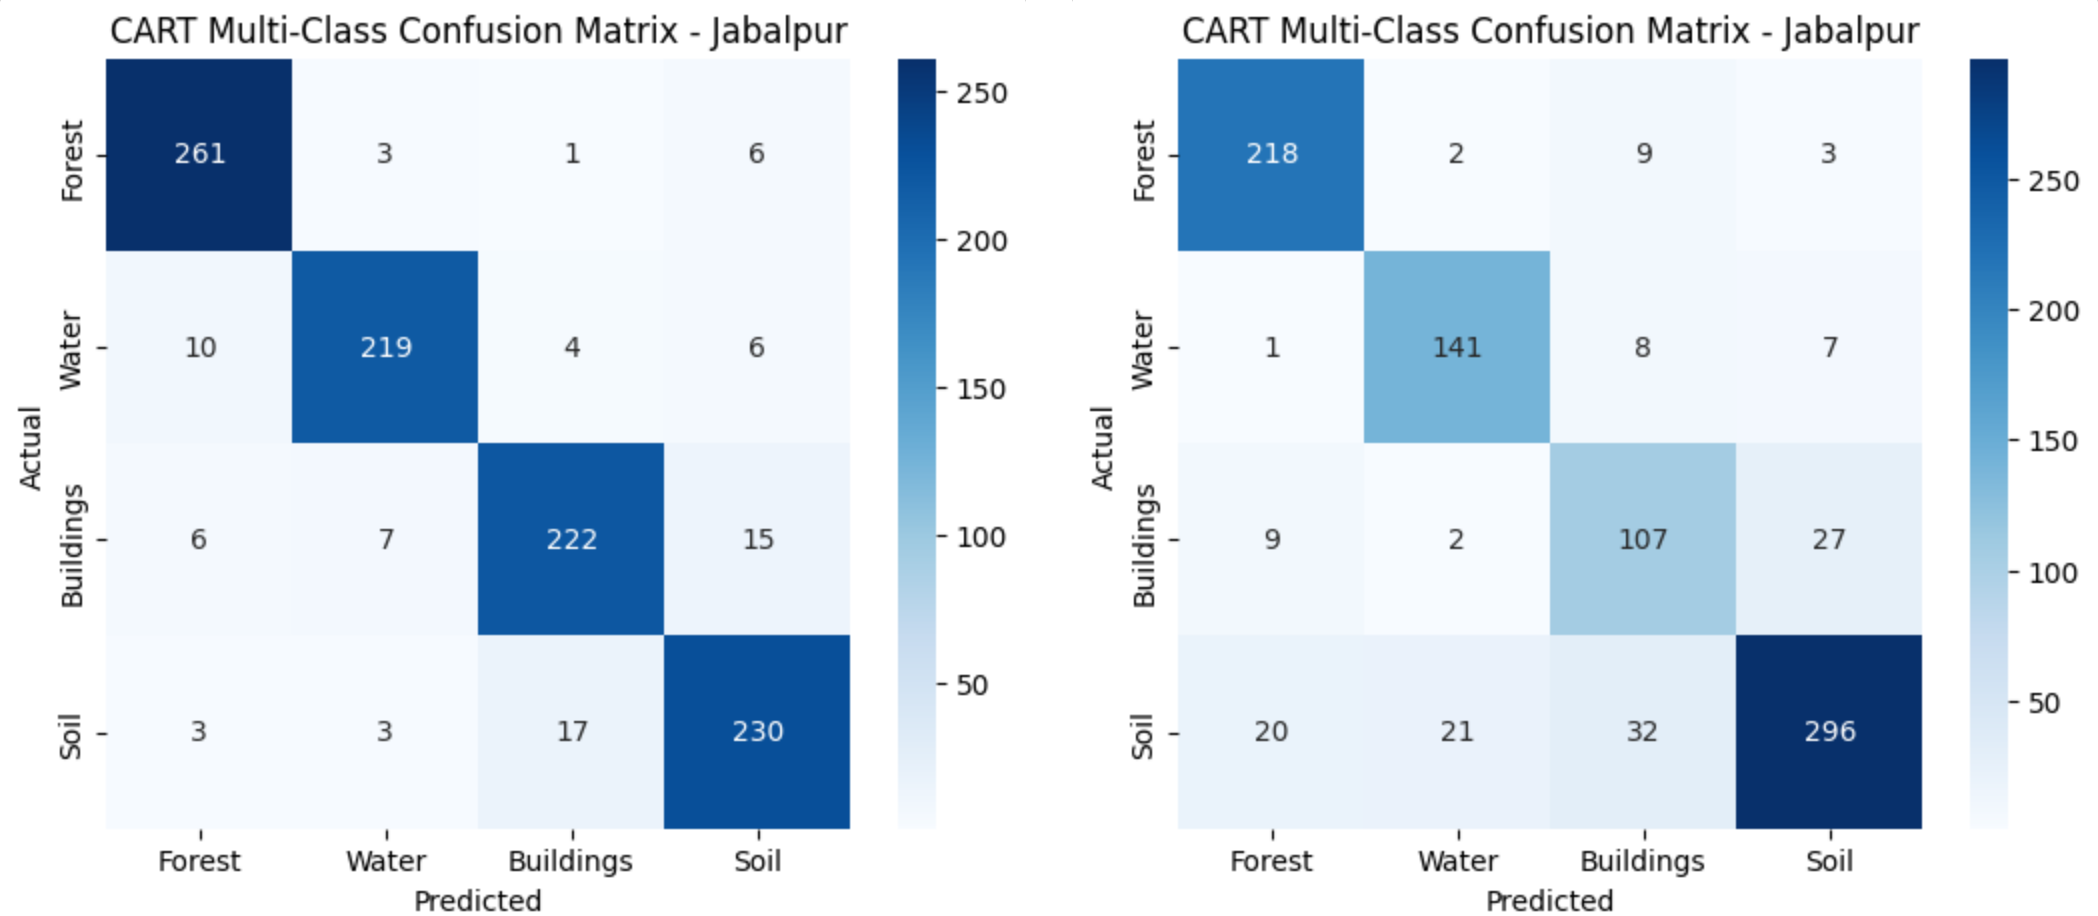
\includegraphics[width=\textwidth]{paper_fig_split_protocol.png}
\caption{The same CART model over the Jabalpur labelled set under two
validation protocols. Left: a random held-out split, 92.0\% overall
accuracy. Right: a spatially blocked split of the identical points,
84.4\%. Neither the model, the features nor the labels differ between
the two panels; only the assignment of points to the test set does.}
\label{fig:split}
\end{figure*}

\begin{table}[!t]
\caption{Reported overall accuracy under three validation protocols}
\label{tab:protocol}
\centering
\footnotesize
\begin{tabular}{@{}p{40mm}p{16mm}p{16mm}@{}}
\toprule
\textbf{Protocol} & \textbf{Scope} & \textbf{Overall} \\
\midrule
Random held-out split & Jabalpur & 94.3\% \\
Spatially blocked split & Jabalpur & 79.2--91.5\% \\
External consensus reference & 48 districts & 61.1--85.0\% \\
\bottomrule
\end{tabular}
\end{table}

The 2.8 to 15.1 point gap between the first two rows is spatial
autocorrelation and nothing else, since the models, features and labels
are identical across the two. Fig.~\ref{fig:split} shows one such pair
directly. Labelled points are collected in
clusters, so under a random split neighbouring 10~m pixels from the same
patch fall on both sides, and each model is evaluated against near
duplicates of its own training rows. Under the blocked split, points are
binned into approximately 11~km cells and whole cells are assigned to
one side. The lower figure is the defensible one. This is consistent
with the wider finding that non-spatial cross-validation systematically
overstates the predictive performance of spatially structured ecological
models \cite{ref21,ref22}.

We record this explicitly because the gap is large enough to change a
study's conclusions. A campus-scale accuracy of 94\% and a statewide
accuracy of 62\% can be produced by the same model on the same day, and
only the second describes what a user of the map receives.

Fig.~\ref{fig:jabalpur} through Fig.~\ref{fig:kanha} show the classifier on five areas at map scale, beginning inside the labelled district and then moving outward from it. Classes are \ckey{cForest}{Forest}, \ckey{cWater}{Water}, \ckey{cBuild}{Buildings}, \ckey{cBarren}{Barren Land} and \ckey{cAgri}{Agriculture}.

\begin{figure*}[!t]
\centering
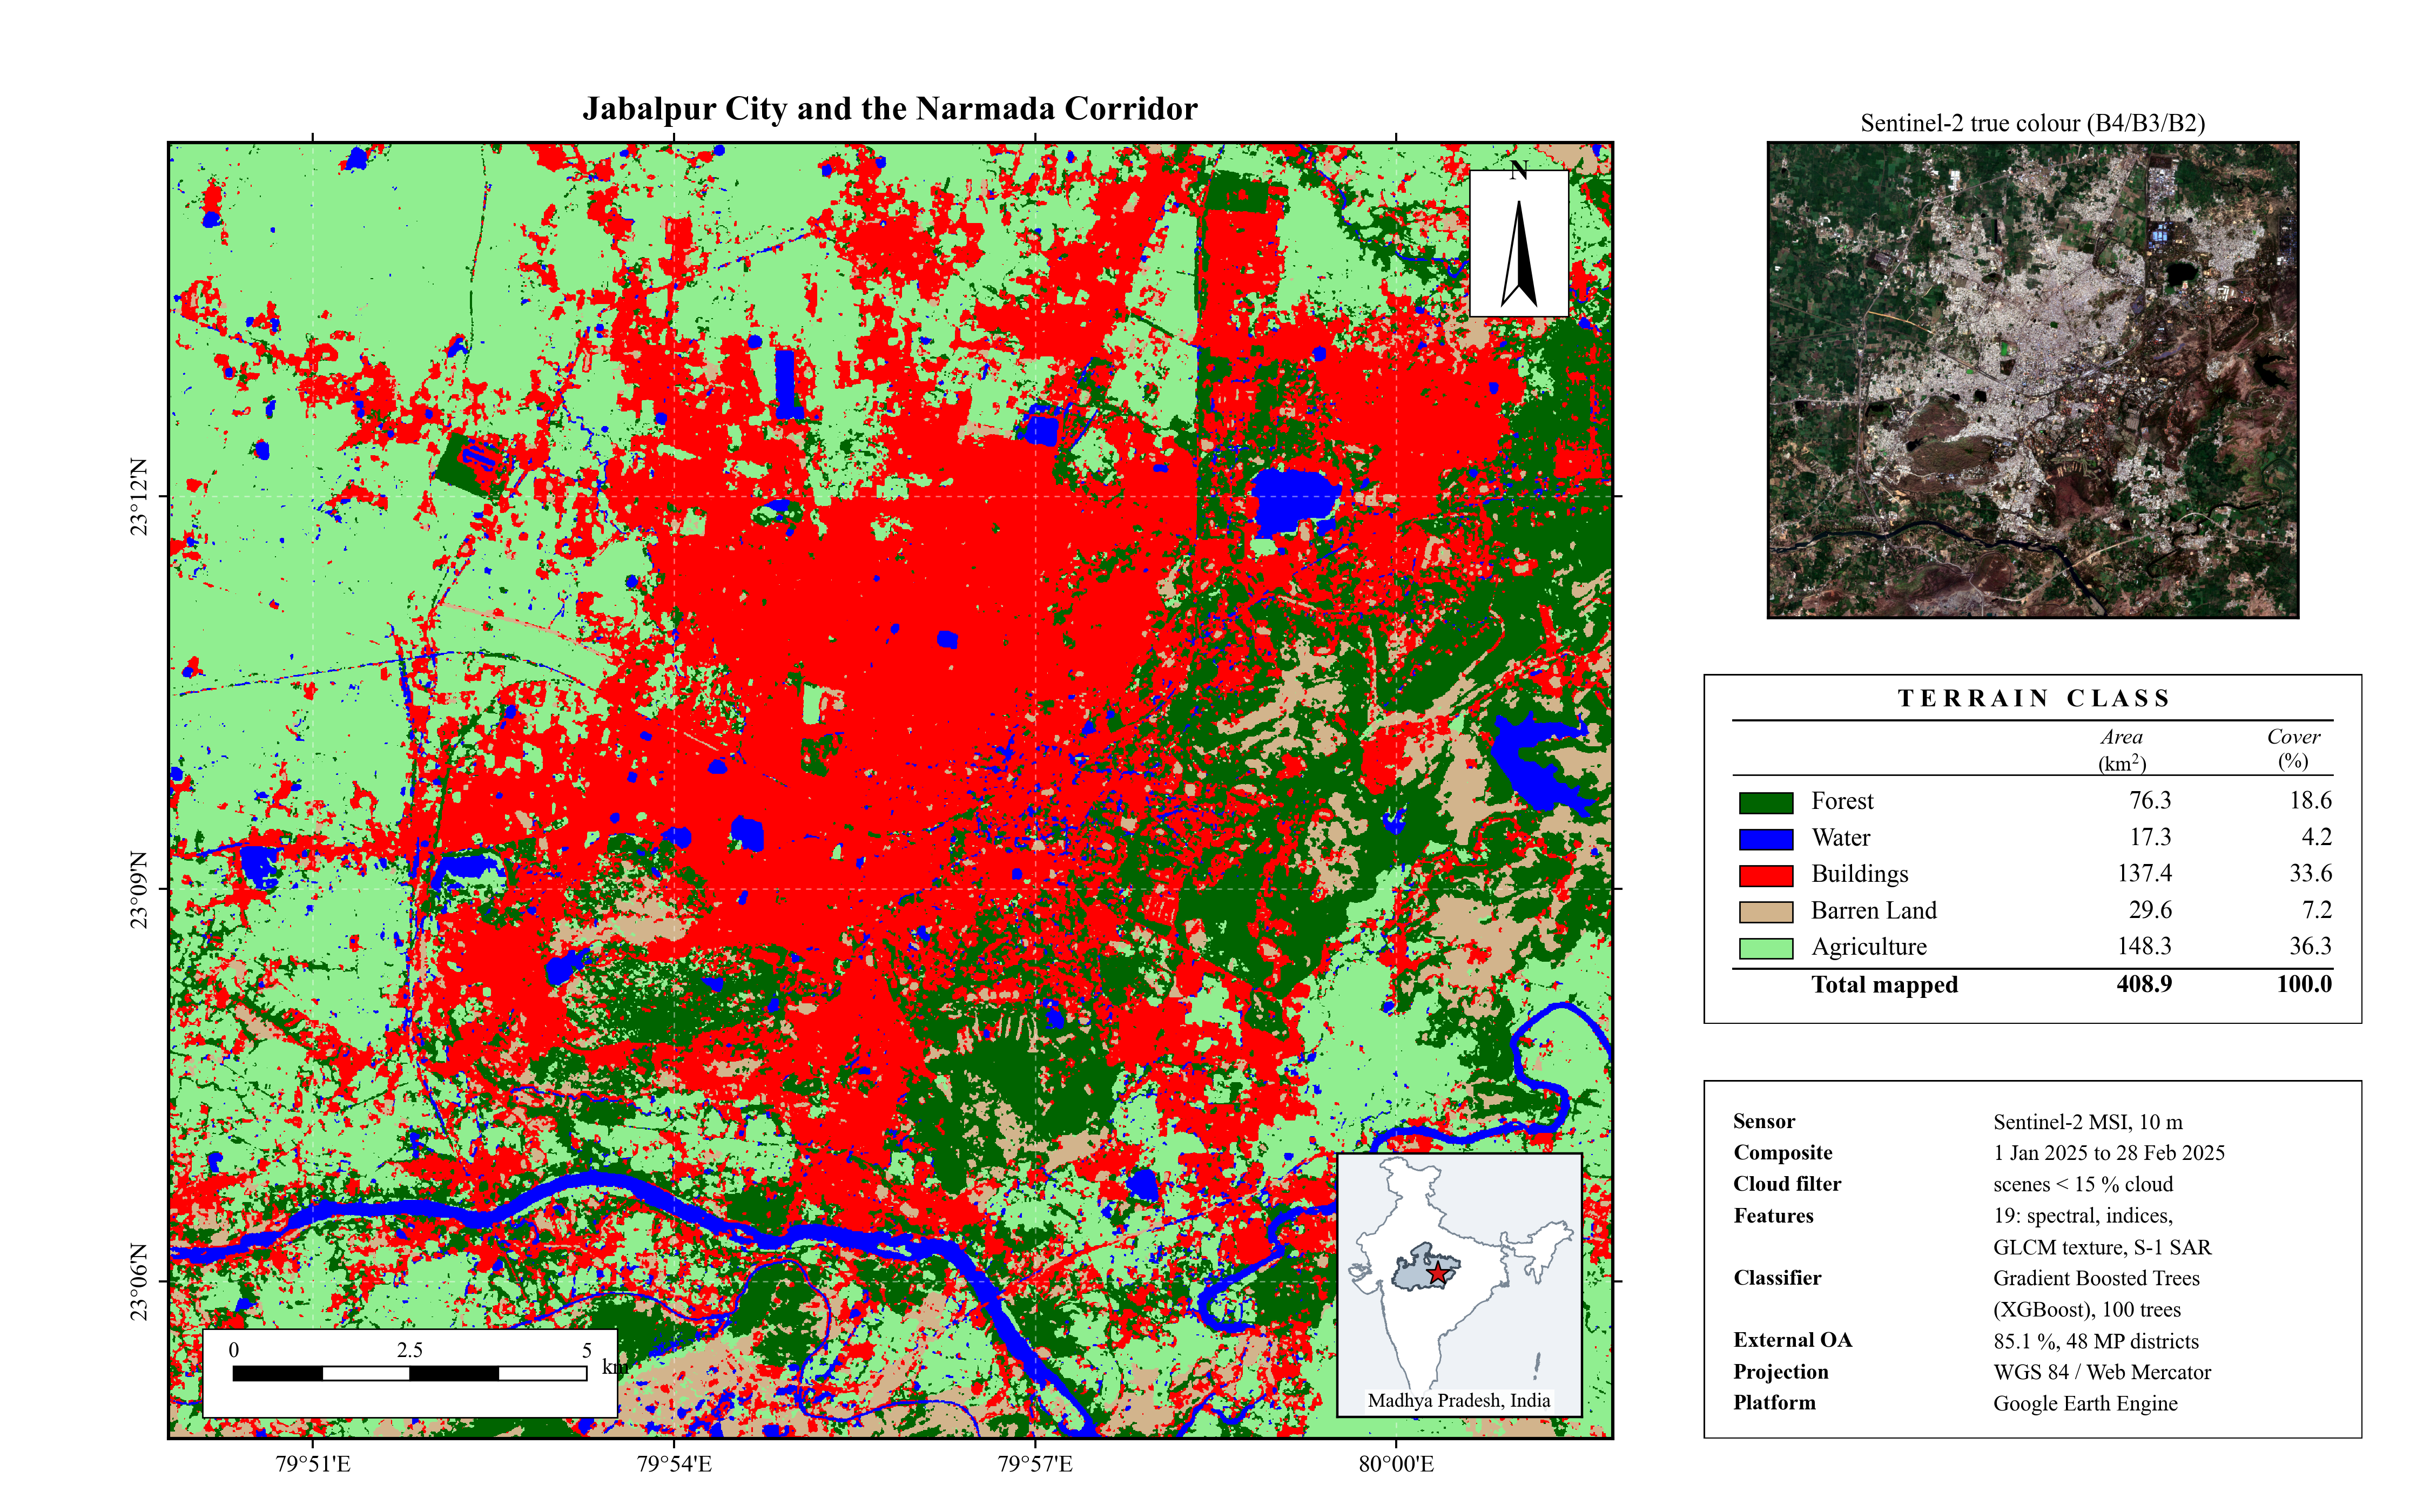
\includegraphics[width=\textwidth]{plate1_jabalpur_city.png}
\caption{Five-class classification of Jabalpur city and the Narmada corridor, inside the district the labelled training set was collected in. Classes are \ckey{cForest}{Forest}, \ckey{cWater}{Water}, \ckey{cBuild}{Buildings}, \ckey{cBarren}{Barren Land} and \ckey{cAgri}{Agriculture}. The built-up core is recovered as one contiguous unit, the Narmada is tracked as an unbroken channel across the southern third of the scene, and the cultivated plain to the north and west separates from the forested ridges on the eastern margin. Every pixel is served by the deployed classifier at 10~m.}
\label{fig:jabalpur}
\end{figure*}
\begin{figure*}[!t]
\centering
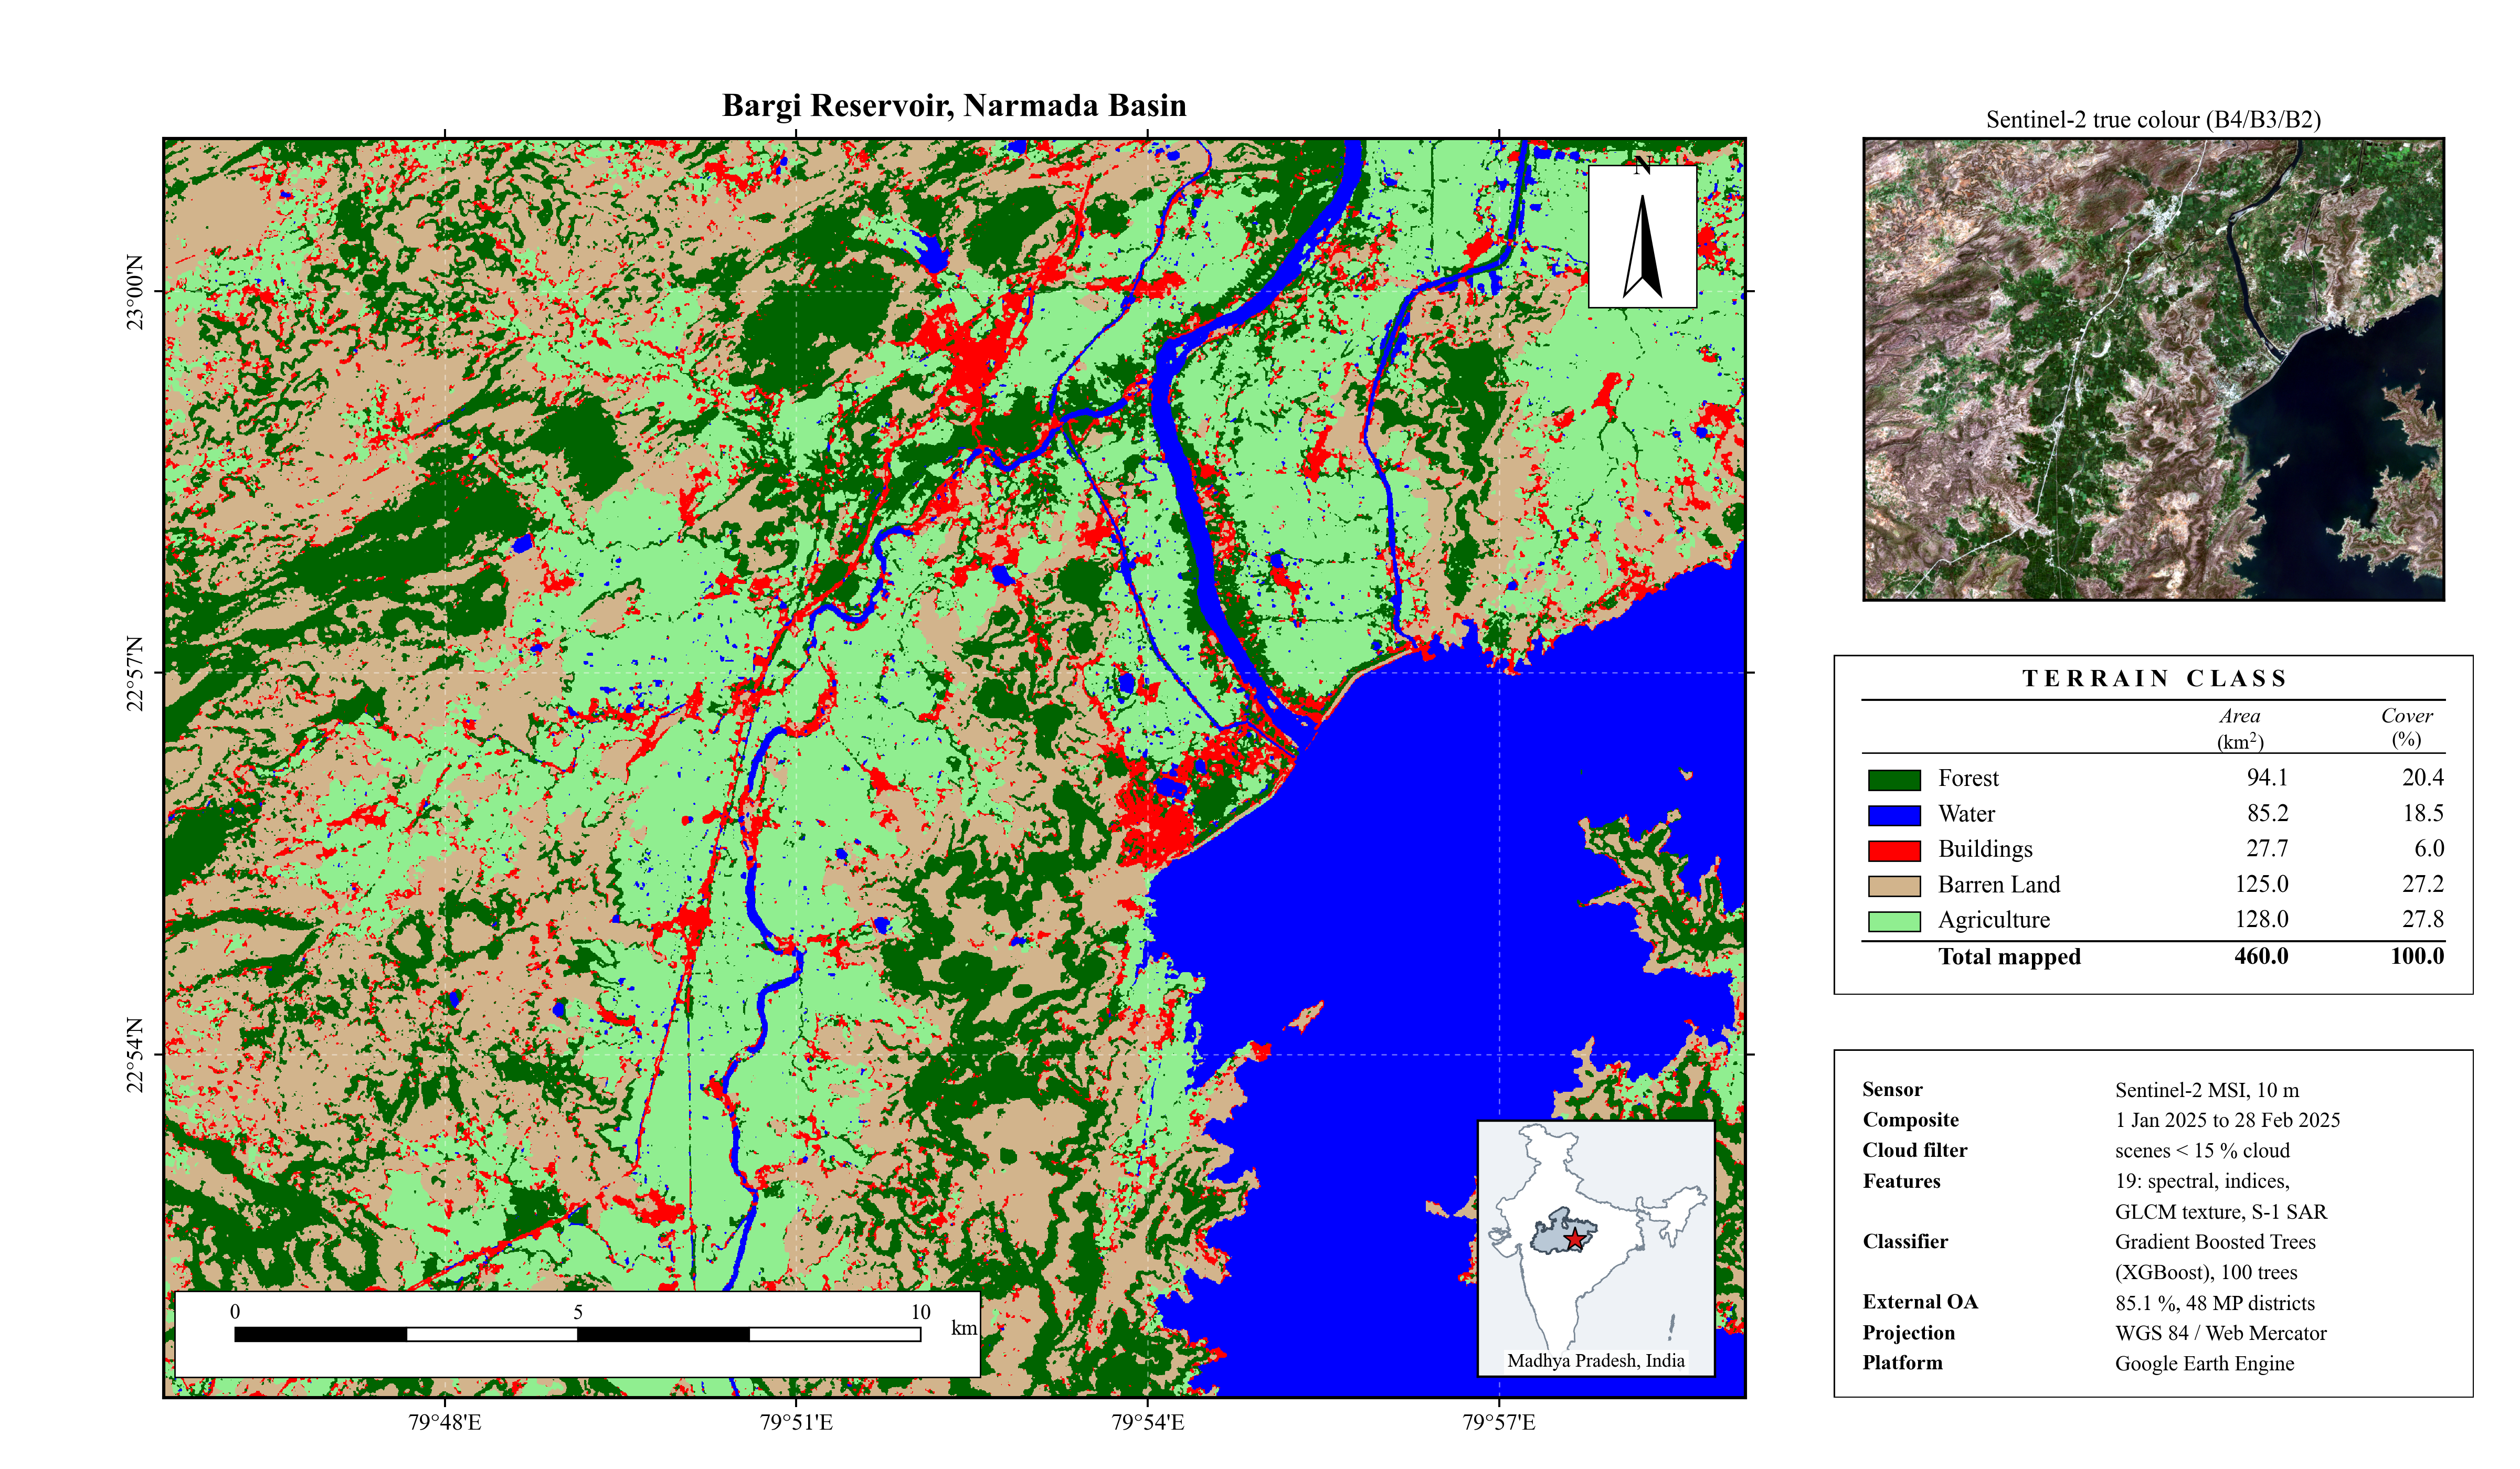
\includegraphics[width=\textwidth]{plate2_bargi_reservoir.png}
\caption{Classification of the Bargi reservoir and its drawdown margin, 40~km south-west of the training area. A large water body with a complex shoreline is the clearest available read on Water precision away from the labelled points.}
\label{fig:bargi}
\end{figure*}
\begin{figure*}[!t]
\centering
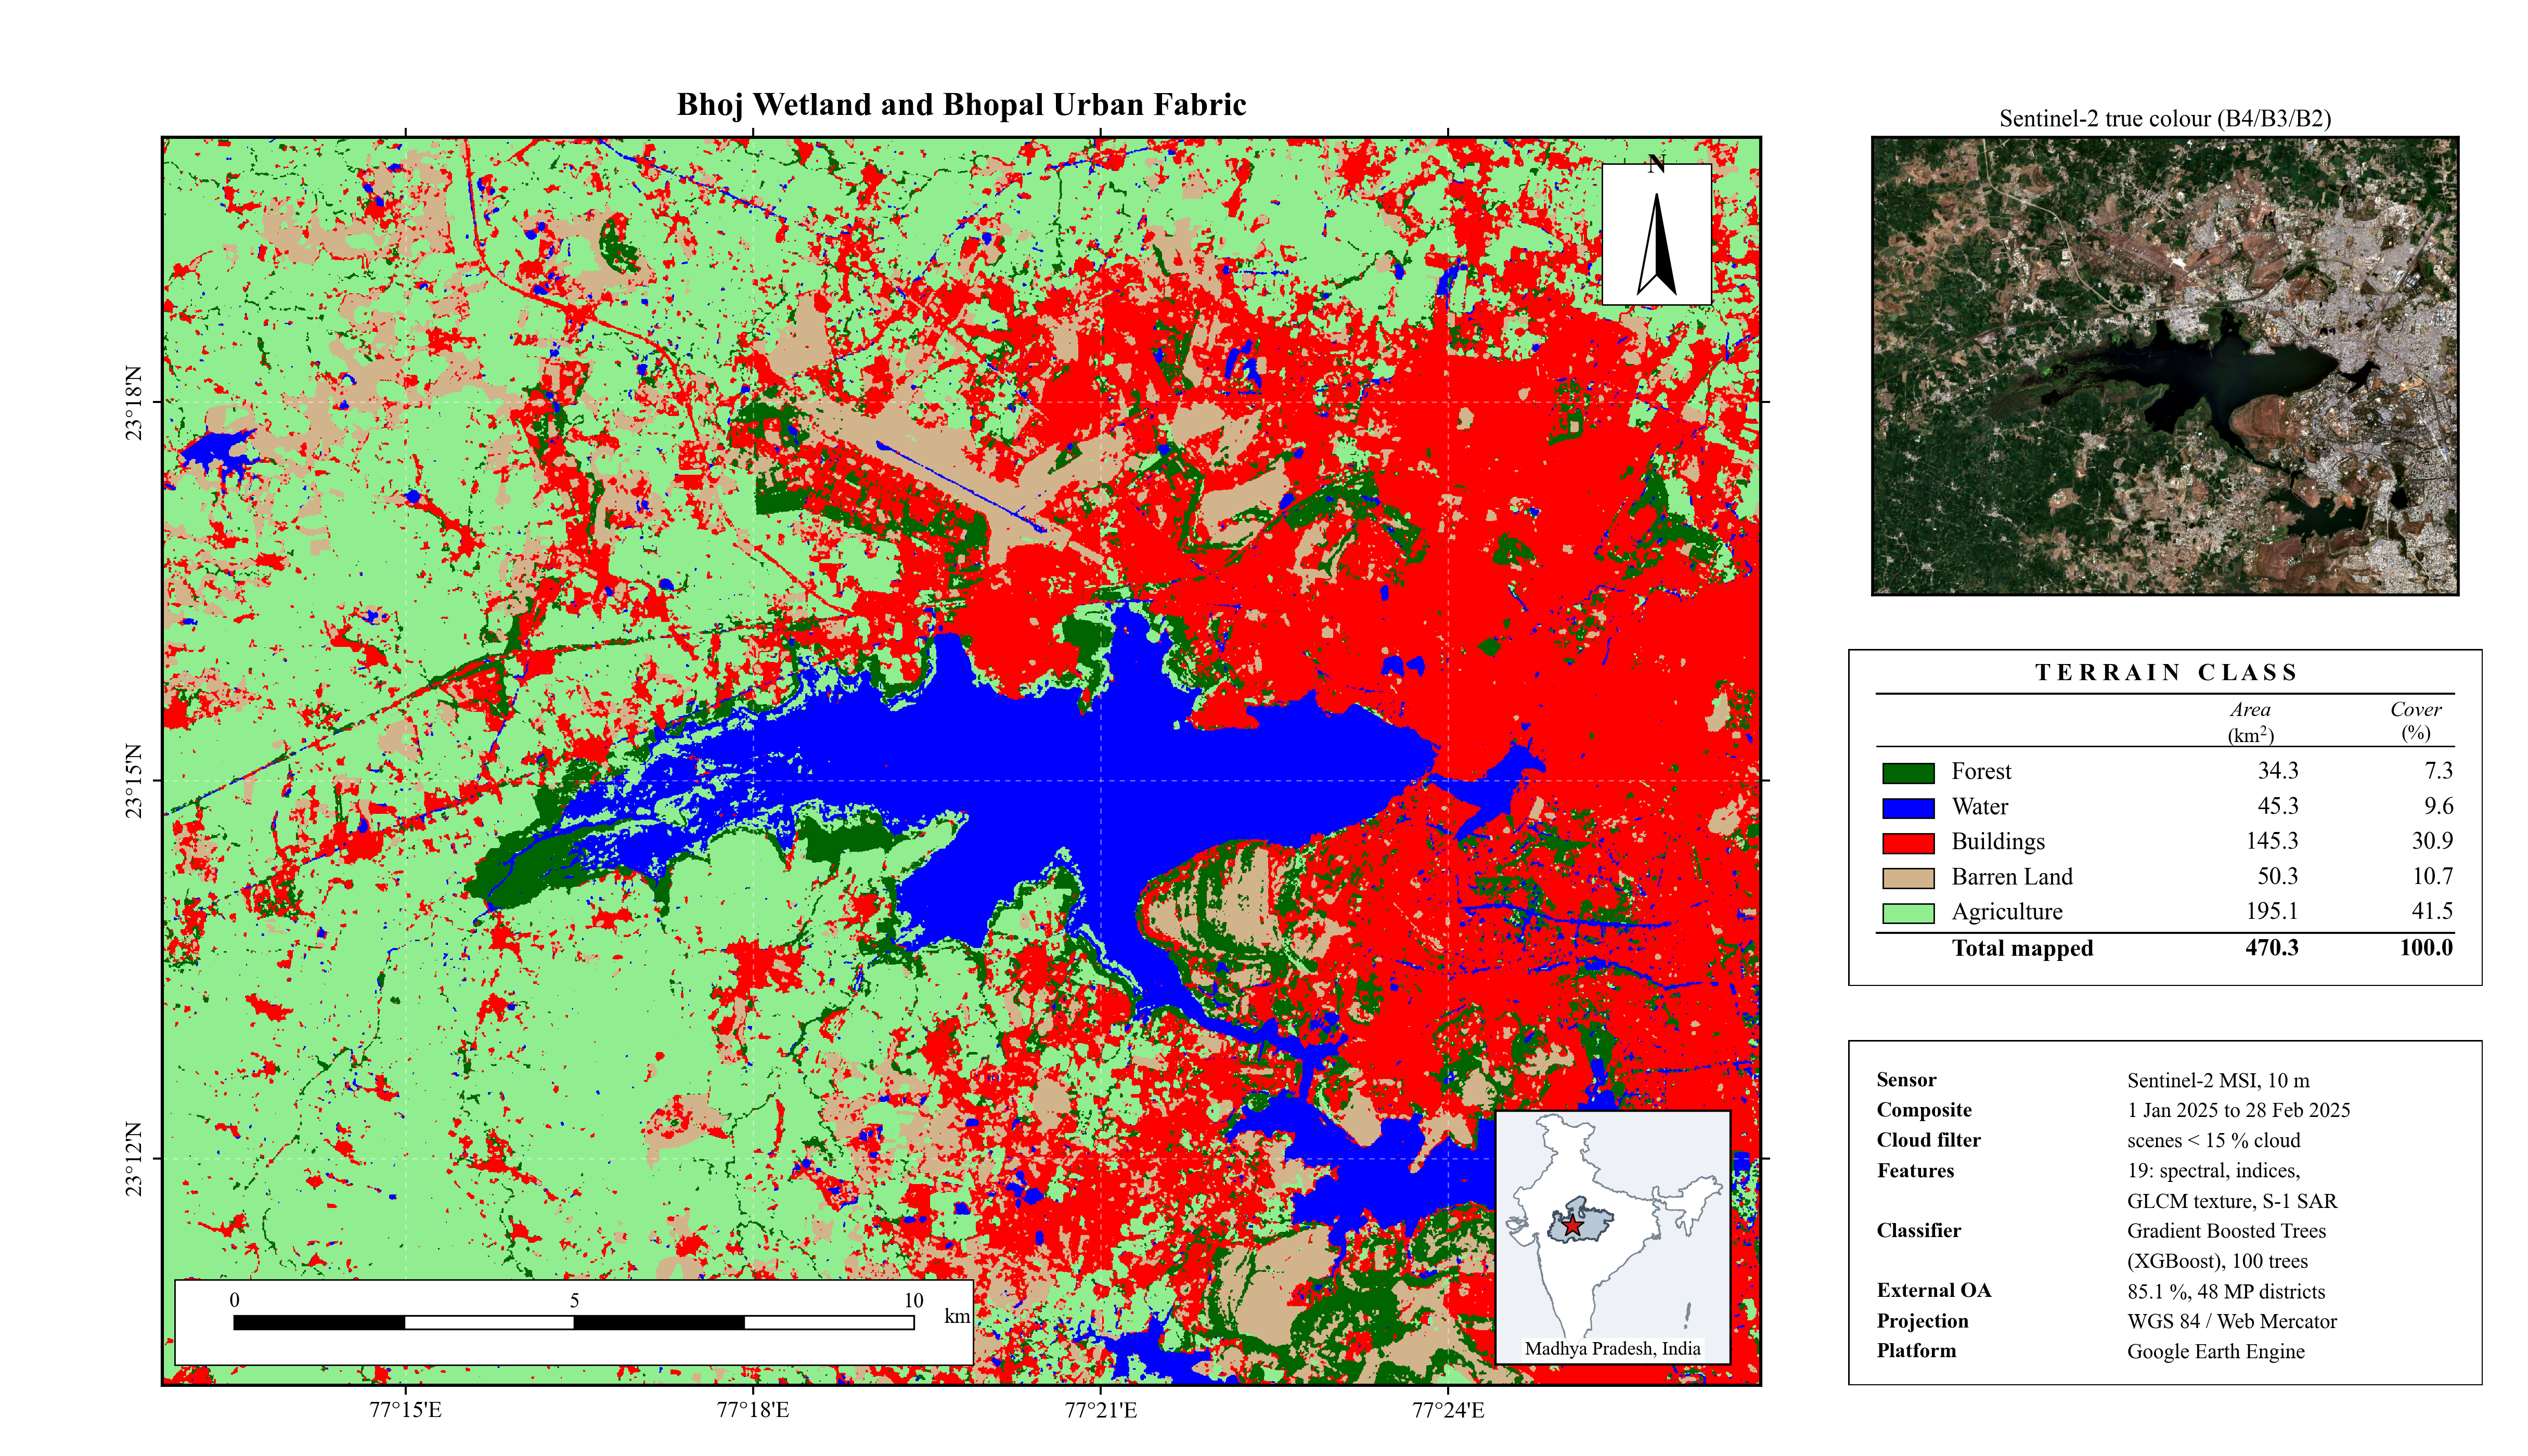
\includegraphics[width=\textwidth]{plate3_bhopal_lake.png}
\caption{Classification of the Upper and Lower Lakes at Bhopal, roughly 300~km west of the training area, where open water and dense urban fabric are adjacent.}
\label{fig:bhopal}
\end{figure*}
\begin{figure*}[!t]
\centering
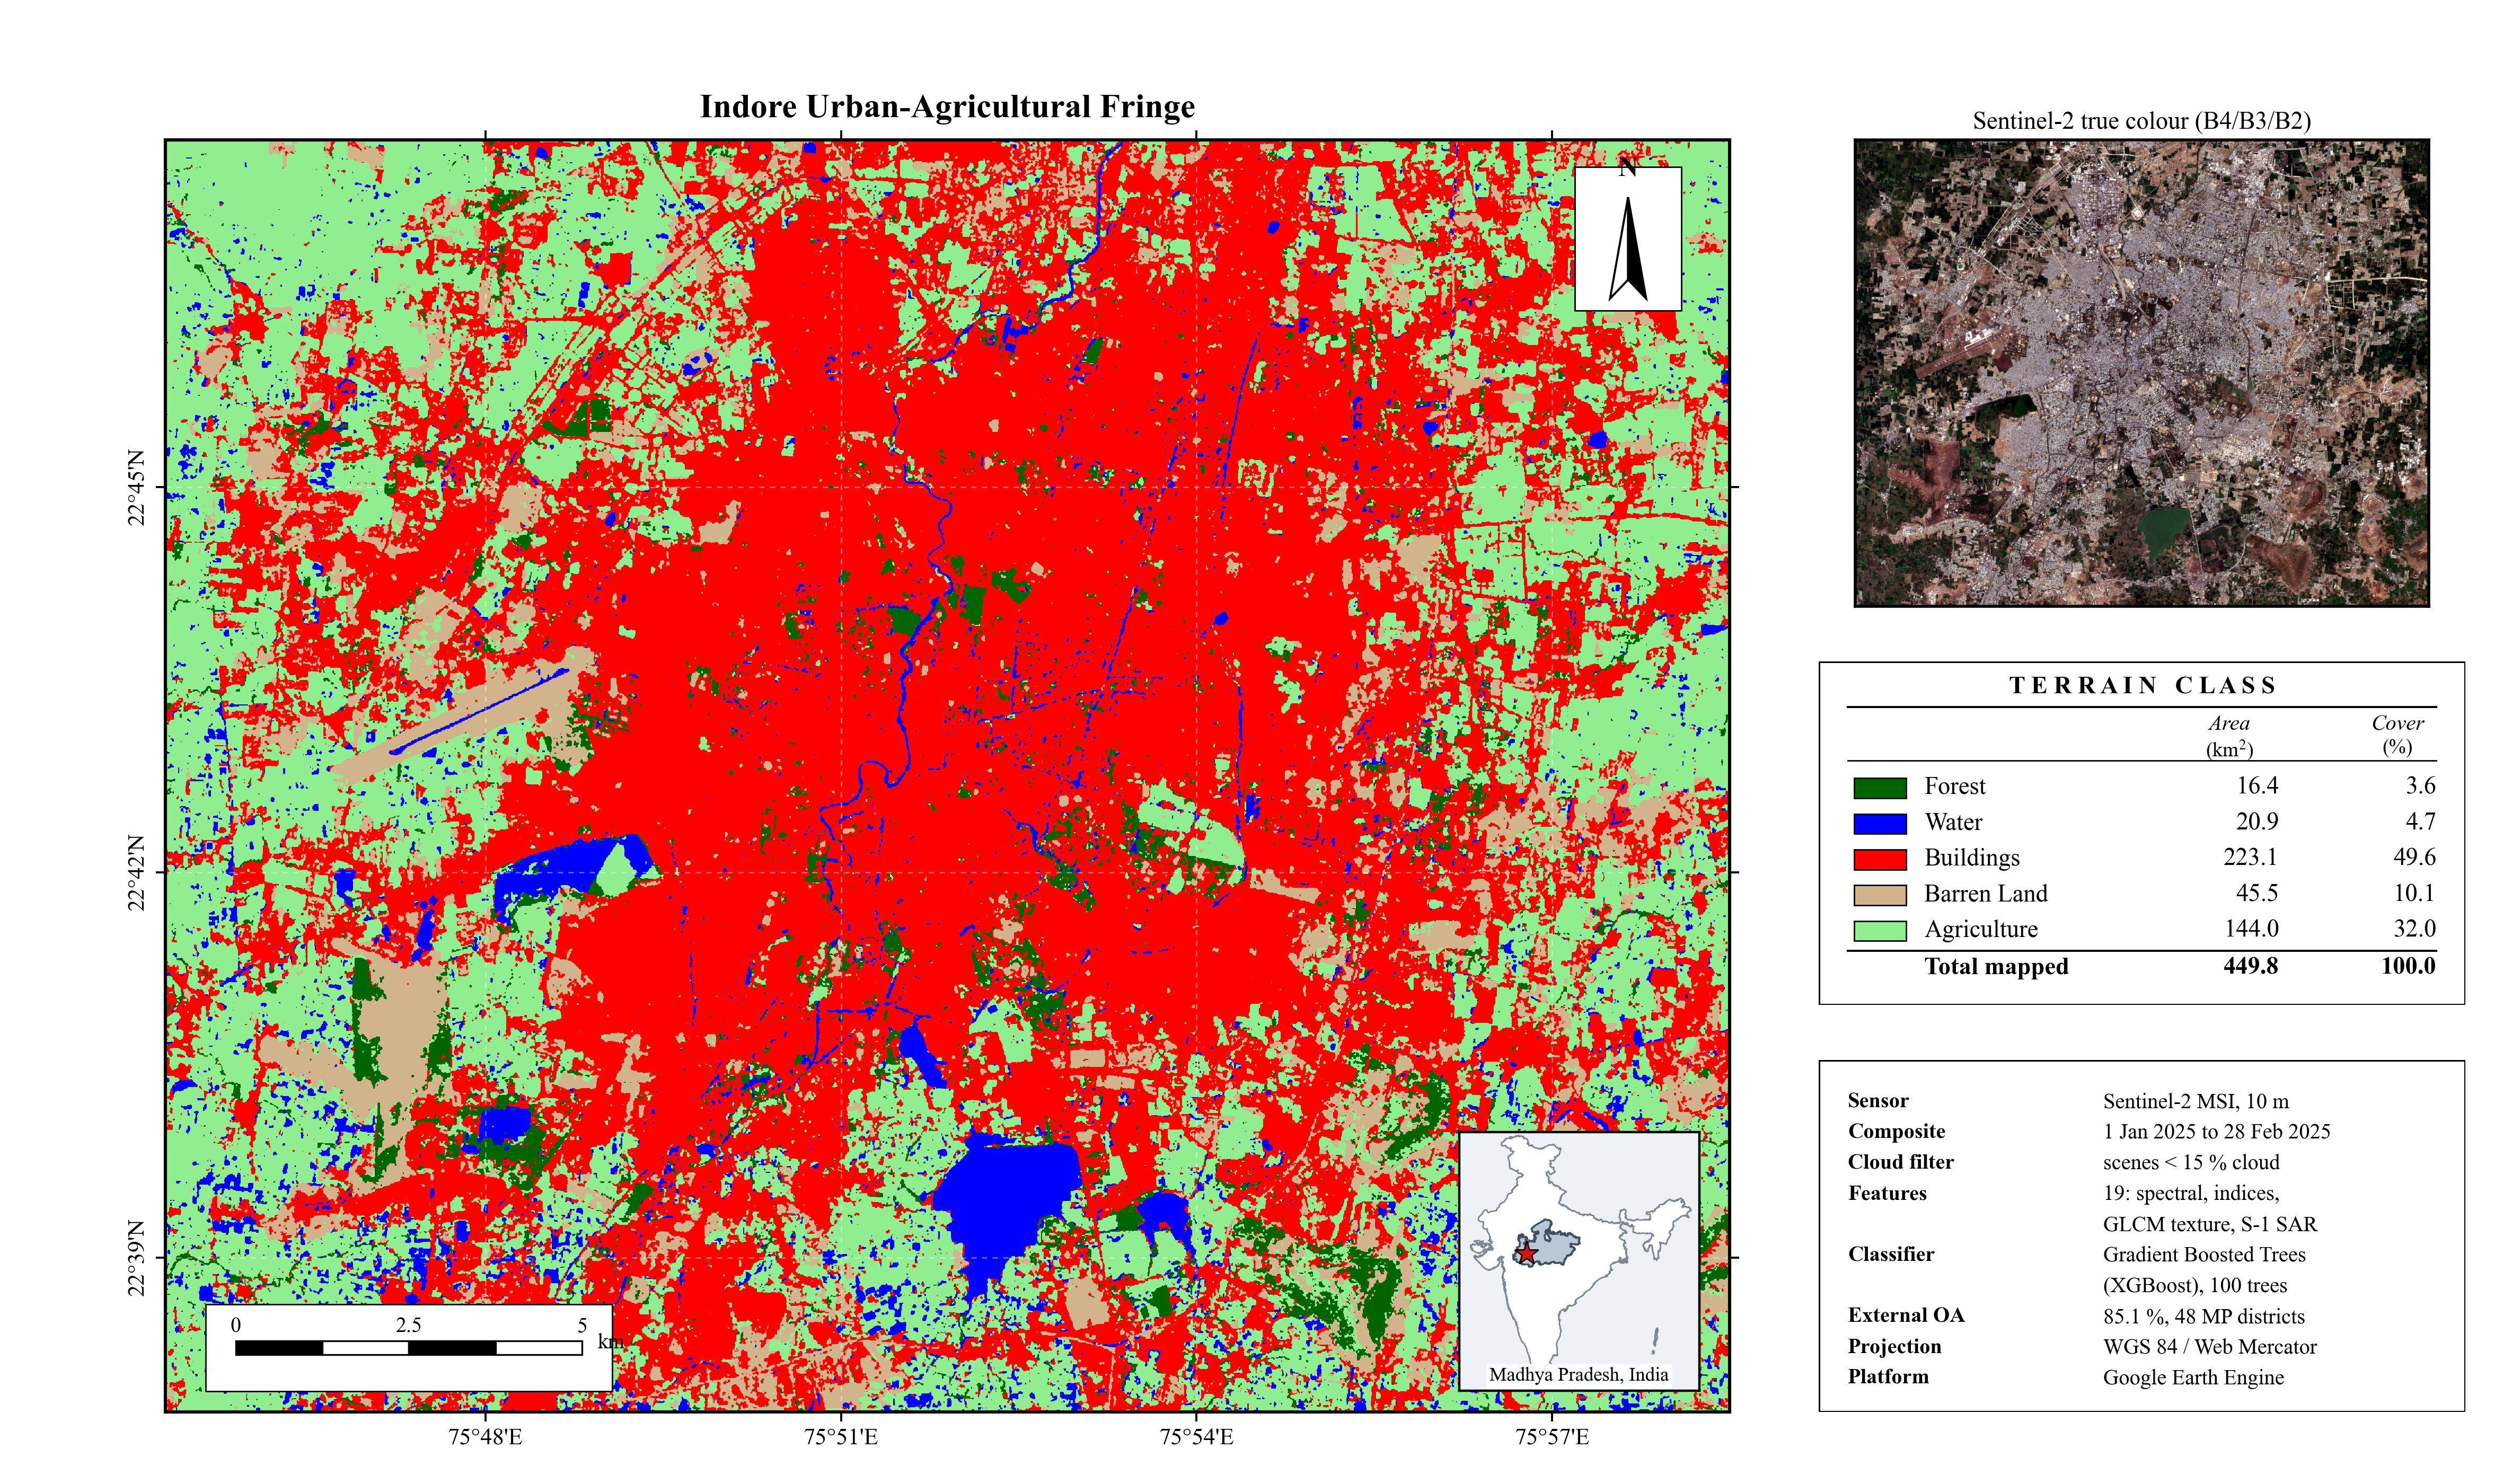
\includegraphics[width=\textwidth]{plate4_indore_fringe.png}
\caption{Classification of the Indore urban fringe, where built-up land meets the black cotton soils of the Malwa plateau. This is the failure case the limitations describe: the terrain has no labelled bare ground in the training set, and the model over-calls Buildings across it.}
\label{fig:indore}
\end{figure*}
\begin{figure*}[!t]
\centering
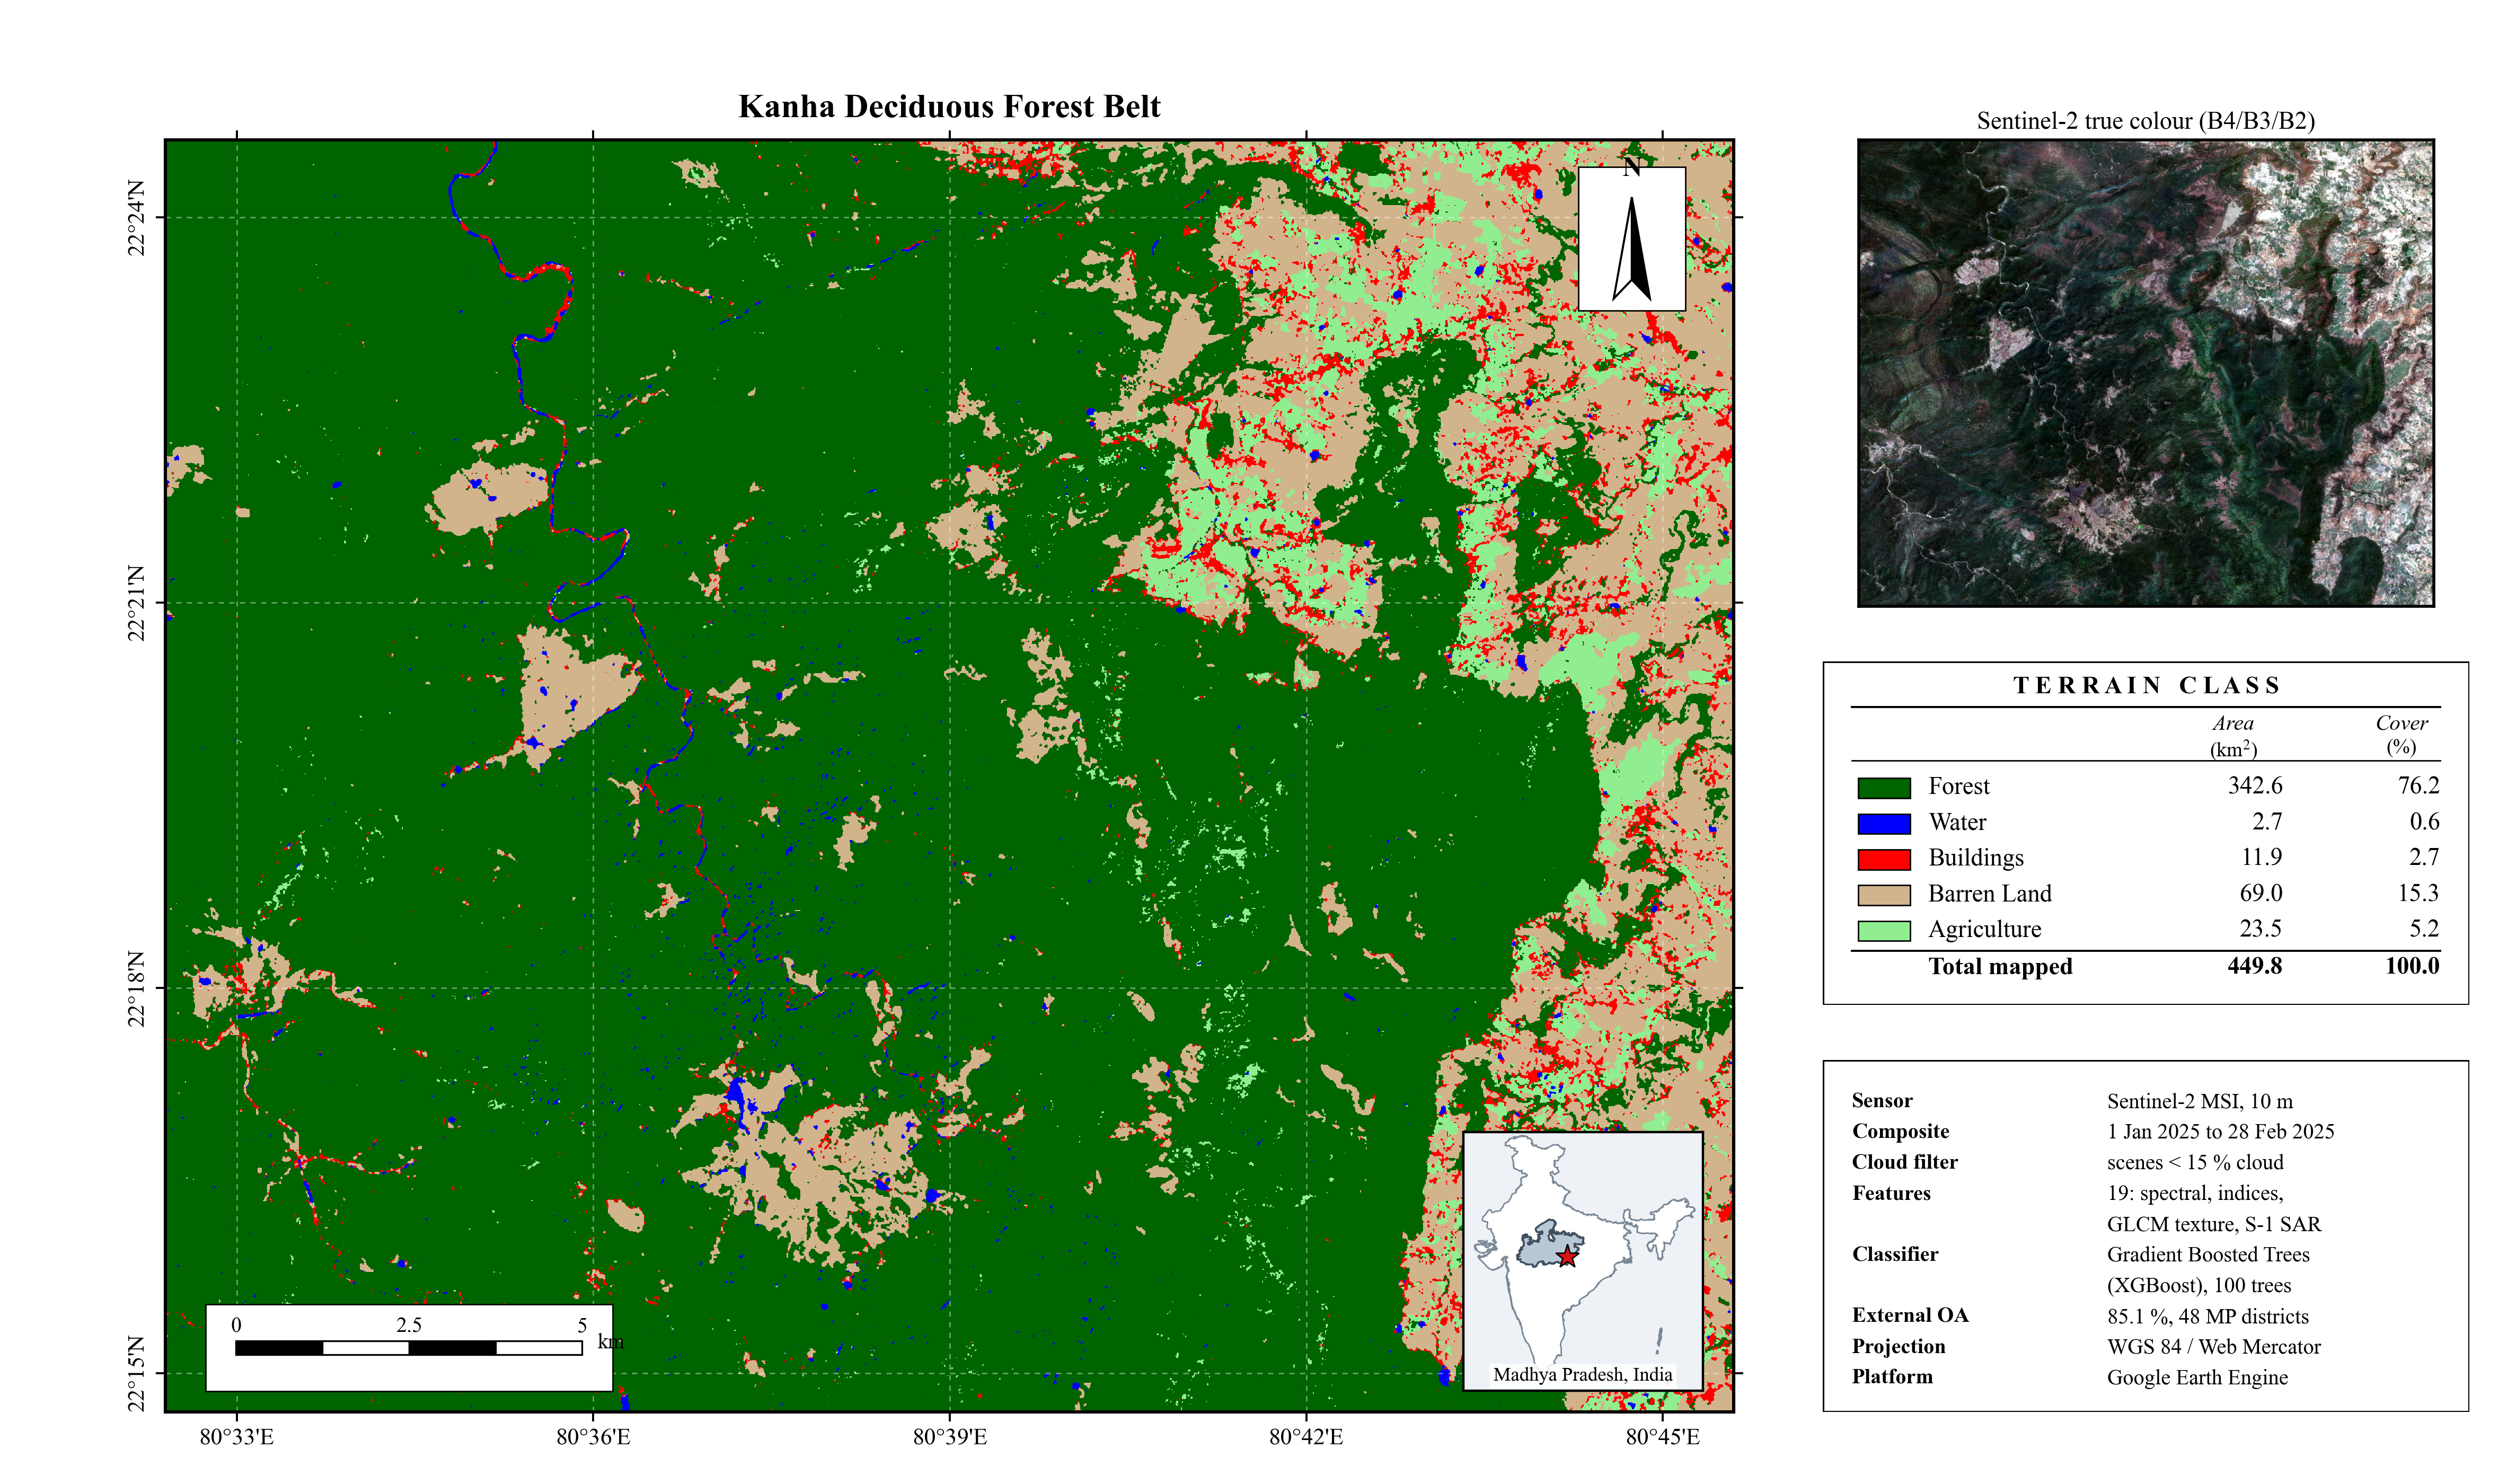
\includegraphics[width=\textwidth]{plate5_kanha_forest.png}
\caption{Classification of the Kanha forest block and the cultivated land along its boundary, the class pair the summer composite separates least well.}
\label{fig:kanha}
\end{figure*}

\section{Limitations}

Five limitations bound the results reported here.

First, the reference is agreement rather than field truth. WorldCover is
itself approximately 75--80\% accurate, and disagreement with it is not
automatically the model's error. The consensus construction of
Section~\ref{sec:reference} is designed to raise reference precision by
masking every pixel on which the products disagree, at the cost of
sampling only the terrain those products find easy, which if anything
flatters all five classifiers equally.

Second, the reference products are temporally mismatched with the 2025
composites. WorldCereal is a 2021 product and the GHSL built surface
layer is 2018, so genuine change since those dates is scored as model
error.

Third, the current inventory sources Barren Land from Jabalpur district
alone. The statewide bare-ground labels that produced the Thar result
above were removed when the class was redefined. Statewide bare-ground
performance is therefore expected to regress relative to that
measurement, and the west-to-east gradient of
Section~\ref{sec:spatial} indicates where.

Fourth, the classifier hyperparameters in Table~\ref{tab:models} were
selected for an earlier four-class problem and have not been re-tuned
for five classes and nineteen features. We previously identified the SVM
$\gamma$ as the likely explanation for its position in the ranking; that
attribution was incorrect, and the cause was the feature scaling
described in Section~\ref{sec:models}. A $\gamma$ of 1.0 is a defensible
value for nineteen unit-scaled features, and it is the value used for
the results reported here, but it has still not been tuned and remains
the most likely remaining source of headroom for SVM.

Fifth, sampling is stratified by reference class rather than by natural
prevalence, so the reported overall accuracies are balanced-class
figures and are not weighted by how common each class actually is across
the state \cite{ref30}.

\section{Conclusion and Future Scope}

This study extended a two-class Sentinel-2 vegetation classification
framework into a five-class terrain classification product evaluated
across an entire Indian state. Three findings are worth carrying
forward.

The bare-versus-built confusion is physical rather than algorithmic, and
it responds to features that carry non-spectral evidence. GLCM texture
repaired the precision half of the confusion and Sentinel-1 radar
repaired the recall half, together taking bare-ground recall from 7\% to
54\% and overall accuracy from 58.6\% to 73.9\%, whereas five additional
bareness indices of the NDBI family contributed 1.8 points between them.
More features are not uniformly better: reducing the stack from 27 bands
to a validated 19 improved Random Forest by 4.5 points on independent
samples and was confirmed on a geographically held-out design.

Under a strict external protocol across 48 districts, XGBoost reached
85.11\% overall accuracy and a Kappa of 0.814 in winter, with SVM and
KNN close behind at 84.10\% and 83.16\%, and Random Forest and CART at
78.04\% and 71.36\%. An earlier version of this work placed the two
distance-based classifiers last. We traced that to GLCM texture bands
entering the stack in raw units and dominating the distance metric on
which those two classifiers alone depend; correcting the scaling moved
them by 12.8 and 9.5 points in winter and left the tree ensembles
within 0.2.

The largest single effects measured anywhere in this work were not model
choices. Changing the validation protocol moved the reported figure by
up to 33 points with no change to the model at all, and labelling
terrain the training set did not represent moved statewide bare-ground
recall by 47 points. Both are properties of the experimental setup and
the training distribution rather than of the algorithm, and both are
easy to report incorrectly.

Future work follows directly from the limitations. Labelling bright arid
and rocky terrain in western Madhya Pradesh addresses the cause of the
district gradient rather than its symptom. A probability reject option,
emitting an explicit unknown class where the maximum class probability
is low, would convert the largest confusion cell into a flagged band
instead of a silent error. A rasterised building-footprint prior offers
geometric evidence that is decorrelated from reflectance. On the radar
side, compositing consistently by relative orbit, normalising for
incidence angle, and adding the temporal standard deviation of the
backscatter would recover separation that the current median composite
discards. Finally, the SVM kernel width should be re-tuned for the
current feature dimensionality before its ranking here is treated as
settled.

\begin{thebibliography}{00}

\bibitem{ref1} J. W. Rouse et al., ``Monitoring vegetation systems in
the Great Plains with ERTS,'' \emph{NASA Special Publication}, vol. 351,
p. 309, 1974.

\bibitem{ref2} C. J. Tucker, ``Red and photographic infrared linear
combinations for monitoring vegetation,'' \emph{Remote Sens. Environ.},
vol. 8, no. 2, pp. 127--150, May 1979, doi:
10.1016/0034-4257(79)90013-0.

\bibitem{ref3} Z. Zhao et al., ``Comparison of three machine learning
algorithms using Google Earth Engine for land use land cover
classification,'' \emph{Rangel. Ecol. Manag.}, vol. 92, pp. 129--137,
Jan. 2024, doi: 10.1016/j.rama.2023.10.007.

\bibitem{ref4} M. Drusch et al., ``Sentinel-2: ESA's optical
high-resolution mission for GMES operational services,'' \emph{Remote
Sens. Environ.}, vol. 120, pp. 25--36, May 2012, doi:
10.1016/j.rse.2011.11.026.

\bibitem{ref5} D. Phiri, M. Simwanda, S. Salekin, V. R. Nyirenda,
Y. Murayama, and M. Ranagalage, ``Sentinel-2 data for land cover/use
mapping: a review,'' \emph{Remote Sens.}, vol. 12, no. 14, 2291, Jul.
2020, doi: 10.3390/rs12142291.

\bibitem{ref7} M. Pal and P. M. Mather, ``Support vector machines for
classification in remote sensing,'' \emph{Int. J. Remote Sens.}, vol.
26, no. 5, pp. 1007--1011, Mar. 2005, doi:
10.1080/01431160512331314083.

\bibitem{ref8} M. Immitzer, F. Vuolo, and C. Atzberger, ``First
experience with Sentinel-2 data for crop and tree species
classifications in central Europe,'' \emph{Remote Sens.}, vol. 8, no. 3,
166, Feb. 2016, doi: 10.3390/rs8030166.

\bibitem{ref9} A. E. Maxwell, T. A. Warner, and F. Fang,
``Implementation of machine-learning classification in remote sensing:
an applied review,'' \emph{Int. J. Remote Sens.}, vol. 39, no. 9, pp.
2784--2817, May 2018, doi: 10.1080/01431161.2018.1433343.

\bibitem{ref10} P. O. Gislason, J. A. Benediktsson, and J. R.
Sveinsson, ``Random forests for land cover classification,''
\emph{Pattern Recognit. Lett.}, vol. 27, no. 4, pp. 294--300, Mar. 2006,
doi: 10.1016/j.patrec.2005.08.011.

\bibitem{ref11} N. Gorelick, M. Hancher, M. Dixon, S. Ilyushchenko,
D. Thau, and R. Moore, ``Google Earth Engine: planetary-scale geospatial
analysis for everyone,'' \emph{Remote Sens. Environ.}, vol. 202, pp.
18--27, Dec. 2017, doi: 10.1016/j.rse.2017.06.031.

\bibitem{ref12} T. Molnár and G. Király, ``Forest monitoring based on
Sentinel-2 satellite imagery, Google Earth Engine cloud computing, and
machine learning,'' Preprint, Jul. 2023, doi:
10.20944/preprints202307.0800.v1.

\bibitem{ref13} F. Razzano, M. R. Iandolo, C. Zarro, G. S. Yogesh, and
S. L. Ullo, ``Integration of Sentinel-1 and Sentinel-2 data for Earth
surface classification using machine learning algorithms implemented on
Google Earth Engine,'' in \emph{Proc. IEEE India Geosci. Remote Sens.
Symp. (InGARSS)}, Aug. 2023, doi: 10.1109/InGARSS59135.2023.10490344.

\bibitem{ref15} L. Breiman, ``Random forests,'' \emph{Mach. Learn.},
vol. 45, no. 1, pp. 5--32, Oct. 2001, doi: 10.1023/A:1010933404324.

\bibitem{ref16} C. Cortes and V. Vapnik, ``Support-vector networks,''
\emph{Mach. Learn.}, vol. 20, no. 3, pp. 273--297, Sep. 1995, doi:
10.1007/BF00994018.

\bibitem{ref17} T. Chen and C. Guestrin, ``XGBoost: a scalable tree
boosting system,'' in \emph{Proc. 22nd ACM SIGKDD Int. Conf. Knowl.
Discov. Data Min.}, Aug. 2016, pp. 785--794, doi:
10.1145/2939672.2939785.

\bibitem{ref18} D. Zanaga et al., ``ESA WorldCover 10 m 2021 v200,''
Zenodo, 2022, doi: 10.5281/zenodo.7254221.

\bibitem{ref19} C. F. Brown et al., ``Dynamic World, near real-time
global 10 m land use land cover mapping,'' \emph{Sci. Data}, vol. 9,
251, Jun. 2022, doi: 10.1038/s41597-022-01307-4.

\bibitem{ref20} R. Torres et al., ``GMES Sentinel-1 mission,''
\emph{Remote Sens. Environ.}, vol. 120, pp. 9--24, May 2012, doi:
10.1016/j.rse.2011.05.028.

\bibitem{ref21} D. R. Roberts et al., ``Cross-validation strategies for
data with temporal, spatial, hierarchical, or phylogenetic structure,''
\emph{Ecography}, vol. 40, no. 8, pp. 913--929, Aug. 2017, doi:
10.1111/ecog.02881.

\bibitem{ref22} P. Ploton et al., ``Spatial validation reveals poor
predictive performance of large-scale ecological mapping models,''
\emph{Nat. Commun.}, vol. 11, 4540, Sep. 2020, doi:
10.1038/s41467-020-18321-x.

\bibitem{ref23} R. M. Haralick, K. Shanmugam, and I. Dinstein,
``Textural features for image classification,'' \emph{IEEE Trans. Syst.
Man Cybern.}, vol. SMC-3, no. 6, pp. 610--621, Nov. 1973, doi:
10.1109/TSMC.1973.4309314.

\bibitem{ref24} Y. Zha, J. Gao, and S. Ni, ``Use of normalized
difference built-up index in automatically mapping urban areas from TM
imagery,'' \emph{Int. J. Remote Sens.}, vol. 24, no. 3, pp. 583--594,
Feb. 2003, doi: 10.1080/01431160304987.

\bibitem{ref25} H. Xu, ``Modification of normalised difference water
index (NDWI) to enhance open water features in remotely sensed
imagery,'' \emph{Int. J. Remote Sens.}, vol. 27, no. 14, pp. 3025--3033,
Jul. 2006, doi: 10.1080/01431160600589179.

\bibitem{ref26} A. Rikimaru, P. S. Roy, and S. Miyatake, ``Tropical
forest cover density mapping,'' \emph{Tropical Ecology}, vol. 43, no. 1,
pp. 39--47, 2002.

\bibitem{ref27} H. Xu, ``A new index for delineating built-up land
features in satellite imagery,'' \emph{Int. J. Remote Sens.}, vol. 29,
no. 14, pp. 4269--4276, Jul. 2008, doi: 10.1080/01431160802039957.

\bibitem{ref28} A. R. Huete, ``A soil-adjusted vegetation index
(SAVI),'' \emph{Remote Sens. Environ.}, vol. 25, no. 3, pp. 295--309,
Aug. 1988, doi: 10.1016/0034-4257(88)90106-X.

\bibitem{ref29} J. Van Tricht et al., ``WorldCereal: a dynamic
open-source system for global-scale, seasonal, and reproducible crop and
irrigation mapping,'' \emph{Earth Syst. Sci. Data}, vol. 15, no. 12, pp.
5491--5515, Dec. 2023, doi: 10.5194/essd-15-5491-2023.

\bibitem{ref30} P. Olofsson, G. M. Foody, M. Herold, S. V. Stehman,
C. E. Woodcock, and M. A. Wulder, ``Good practices for estimating area
and assessing accuracy of land change,'' \emph{Remote Sens. Environ.},
vol. 148, pp. 42--57, May 2014, doi: 10.1016/j.rse.2014.02.015.

\bibitem{ref31} A. Rasul et al., ``Applying built-up and bare-soil
indices from Landsat 8 to cities in dry climates,'' \emph{Land}, vol. 7,
no. 3, 81, Jul. 2018, doi: 10.3390/land7030081.

\end{thebibliography}

\end{document}
